\chapter{ExProSE}
\label{cha:exprose}

This chapter describes ExProSE, a computational method based on distance geometry that generates an ensemble of protein structures from two input structures.
The structures span conformational space and the ensemble generation procedure can be perturbed to predict allosteric sites.
The work is further described in \cite{Greener2017}.


\section{Materials and Methods}
\label{sec:exprose_methods}

ExProSE is based on the CONCOORD distance geometry method \cite{DeGroot1997} and consists of a two-step process of (i) converting interactions in one or more crystal structures into distance constraints and (ii) generating new structures from these constraints.
ExProSE has important differences to CONCOORD that make it suitable for modelling conformational transitions and ensemble perturbations.
These are primarily the use of two input structures instead of one, a different procedure for achieving convergence, the ability to predict the effect of a modulator and an auto-parameterisation procedure.
The effect of a potential modulator can be explored by adding new distance constraints arising due to the modulator and generating new structures with these additional constraints. The original ensemble and the ensemble generated with the extra constraints can then be compared to see how the modulator affects the protein.

ExProSE is implemented in Julia, a language that combines readable syntax similar to Python with performance approaching statically-compiled languages like C.
Work was initially begun in a combination of Python and C++ before switching to Julia.
Use of Julia allows good computational performance at the limiting steps, but also allows compact and easy-to-use code that others can modify.
The code, documentation, details of the datasets and instructions for reproducing the data are freely-available under the MIT license as a Julia package at \url{https://github.com/jgreener64/ProteinEnsembles.jl}.
The code is written in a modular way with associated unit tests and an automated building and testing procedure.


\subsection{Distance constraint generation}

The first step is to obtain a set of distance constraints from a protein structure.
Files for selected structures were obtained from the PDB.
Contrary to similar studies \cite{Panjkovich2012, Huang2013} the smallest biological assembly of the protein is used, rather than only the chain containing the allosteric modulator.
For each protein structure, interatomic distances are calculated from the PDB coordinates.
Hetero atom records, including the allosteric modulators, are removed.
Any existing hydrogens are removed and polar hydrogens are added using an in-house script.
For disordered atoms the location with the highest occupancy in the PDB is selected.
Secondary structure assignments, required to obtain additional distance constraints, are obtained using the DSSP software \cite{Touw2015}.
As two structures for the same protein are utilised to generate distance constraints, only atoms common to both structures are used.
Every atom pair is examined and assigned an interaction type.
The criteria for each interaction are the same as in CONCOORD \cite{DeGroot1997} and are shown in Table~\ref{tab:interaction_types}.


\begin{sidewaystable}
\centering

\begin{small}
% Table generated by Excel2LaTeX from sheet 'interactions'
\begin{tabular}{ l l l p{10cm} }
\hline
\textbf{Number} & \textbf{Interaction name} & \textbf{Constraint tolerance / \AA} & \textbf{Definition} \\
\hline
1  & Covalent bond       & 0.02 & Pairs that are covalently bonded \\
2  & Bond angle          & 0.05 & Pairs where both atoms are covalently bonded to the same atom \\
3  & Ring                & 0.1  & Pairs that are part of ring systems \\
4  & Double bond 1-4     & 0.1  & 1-4 dihedral angle restricted pairs in side chain double bonds (found in ASN, GLN and ARG) \\
5  & Omega 1-4           & 0.1  & 1-4 pairs constrained by the rigid \textomega\ dihedral angle \\
6  & Tight phi/psi 1-4   & 0.2  & 1-4 pairs constrained by the \textphi /\textpsi\ dihedral angle where one residue is a proline or both residues are in the same helix/strand \\
7  & Loose phi/psi 1-4   & 0.4  & 1-4 pairs constrained by the \textphi /\textpsi\ dihedral angle where one residue is a glycine or both residues are in a loop region \\
8  & Other phi/psi 1-4   & 0.3  & 1-4 pairs constrained by the \textphi /\textpsi\ dihedral angle that do not fall into the above two categories \\
9  & Other 1-4           & 0.4  & Other 1-4 dihedral angle restricted pairs that do not fall into the above categories \\
10 & Secondary structure & 0.5  & Pairs of backbone atoms that are in the same helix/strand and are not more than 4 residues apart \\
11 & Salt bridge         & 0.75 & Pairs from oppositely-charged groups in close proximity (less than 4 \AA\ apart) \\
12 & Hydrogen bond       & 0.5  & Pairs that are part of a hydrogen bond; donor-acceptor distance is no more than 3.5 \AA, hydrogen-acceptor distance is no more than 2.5 \AA\ and the donor-hydrogen-acceptor angle is at least 90 degrees \\
13 & Tight hydrophobic   & 0.5  & Pairs where the interatomic distance is less than the sum of the van der Waals radii of the atoms plus 0.5 \AA; only C and H atoms are counted \\
14 & Loose hydrophobic   & 1    & Pairs where the interatomic distance is less than the sum of the van der Waals radii of the atoms plus 1.0 \AA; only C and H atoms are counted \\
15 & All other pairs     & 5    & Pairs that do not fall into any of the above categories \\
\hline
\end{tabular}
\end{small}

\caption{Interaction types between atom pairs.
These are the same as in CONCOORD \cite{DeGroot1997}.
The constraint tolerance values are used to generate lower and upper distance constraints between atoms.}

\label{tab:interaction_types}
\end{sidewaystable}


Each atom pair is assigned the first interaction for which it fulfils the criterion.
If an atom pair is not assigned any of the first 14 specific interactions, it is assigned the generic `All other pairs' interaction type.
Lower and upper distance constraints $l_{ij}$ and $u_{ij}$ are generated for each atom pair $ij$ based on the interatomic distance $d_{ij}$, the constraint tolerance for the interaction $t_{ij}$ and a tolerance weighting factor $W_{B}$ that is between 0.0 and 1.0:

$$
l_{ij} = d_{ij} - W_{B} t_{ij}, \quad u_{ij} = d_{ij} + W_{B} t_{ij}
$$

The justification for and selection of $W_{B}$ is described below.
For example two atoms 1.54 \AA\ apart and in a covalent bond with $W_{B}$ equal to 0.5 would have a lower distance constraint of 1.53 \AA\ and an upper distance constraint of 1.55 \AA, as the constraint tolerance multiplied by $W_{B}$ is 0.01 \AA.
This process yields a set of distance constraints for each crystal structure of a protein.

The distance constraints generated from the two structures for the same protein are combined to get a set of combined constraints.
This is shown visually in Figure~\ref{fig:distance_constraints}.
The constraints are combined in such a way that the new constraints for a given atom pair cover the distance of both the individual constraints for that pair.
For example if two atoms have a lower and upper distance constraint of 6.0 \AA\ and 7.0 \AA\ in structure one, and 6.5 \AA\ and 7.5 \AA\ in structure two, then the new constraints will be 6.0 \AA\ and 7.5 \AA.


\begin{figure}
\centering

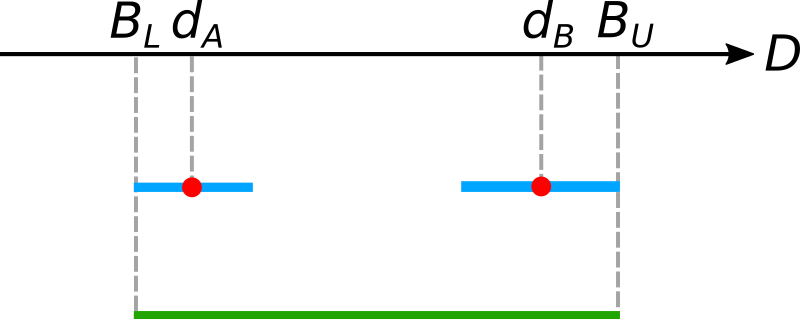
\includegraphics[width=0.6\textwidth]{figures/distance_constraints/distance_constraints}

\caption{The method to calculate the upper and lower distance constraints between two atoms given two input protein structures.
First, the distance between the two atoms in each of the two input structures is calculated ($d_{A}$ and $d_{B}$).
An upper and lower distance constraint is then calculated for each of these distances by multiplying the constraint tolerance for the interaction in that structure by the tolerance weighting factor (these constraints are shown as blue bars).
The upper and lower limits of these constraints are combined to get the new distance constraints $B_{U}$ and $B_{L}$ (green bar).}

\label{fig:distance_constraints}
\end{figure}


It is undesirable to retain all the `All other pairs' interactions (type 15 in Table~\ref{tab:interaction_types}) as they vastly outnumber the specific interactions (types 1-14).
Specific interactions scale with the atom number $N_{A}$ whereas other pairs scale as $N_{A}^{2}$.
Hence only a fraction of the other pairs are retained as distance constraints.
The probability of retaining an other pair is chosen so that the final number of other pairs is roughly $20N_{A}$, the value used by studies utilising CONCOORD \cite{DeGroot1999}.

The parameter $W_{B}$ determines how much the structures are allowed to vary from the input structures.
$W_{B}$ is chosen for each protein in the apo/holo and allosteric datasets by a process of auto-parameterisation.
$W_{B}$ equal to 0.0 usually results in a narrow range of structures that are midway between the two input structures.
By contrast, $W_{B}$ equal to 1.0 usually results in structures that cover a wide conformational space beyond the input structures.
A measure for the conformational spread of the ensemble was developed.
This measure $F$ is the fraction of structures $S$ in the ensemble for which $TM(S,A) > TM(B,A)$ and $TM(S,B) > TM(A,B)$ where $TM(X,Y)$ is the TM-score between model $X$ and reference $Y$, and $A$ and $B$ are the two input crystal structures.
The TM-score is a measure of similarity between two protein structures, with a higher score indicating more similar structures.
$F$ therefore gives the proportion of structures that are closer to both input structures than the input structures are to each other.
$F$ equal to 0.9 indicates an ensemble that effectively covers the conformational space of the input structures.
Ensembles of 50 structures are generated with $W_{B}$ starting at 1.0 and decreasing in steps of 0.1.
When the ensemble generated has an $F$ value of at least 0.9, that $W_{B}$ is chosen.
For the specific examples T4-lysozyme and CDK2, $W_{B}$ is equal to 0.2 and 0.3 respectively.
It should be noted that the above auto-parameterisation procedure to select $W_{B}$ can be implemented automatically by the ExProSE software and requires no input by the user.
For CAP only one input structure is used so $W_{B}$ is selected manually as 0.4.
% NtrC?
This value allows flexibility in the ensemble whilst giving good quality structures.


\subsection{Protein structure generation}

Once the distance constraints have been generated, an iterative process is used to generate structures that satisfy the constraints.
CONCOORD uses a procedure where an atom pair violating a constraint is moved together or apart such that the new distance between the atoms falls randomly within the allowed region.
A new procedure was used here that was found to provide better convergence when utilising combined distance constraints from two structures.
Stochastic Proximity Embedding (SPE) \cite{Agrafiotis2013} was selected, as it has been shown to converge effectively and scales well with system size.
This procedure provides better convergence than the CONCOORD procedure of moving atoms to a random distance within the distance constraints.
The pseudocode for the SPE algorithm, rephrased from an existing review \cite{Agrafiotis2013}, is shown in Algorithm~\ref{algorithm:spe}.
The distance constraints do not include favourability for a particular chirality, so coordinates produced from SPE are examined and structures with the incorrect chirality are reversed by mirroring all coordinates in the $xy$ plane.


\begin{algorithm}[p]
\caption{SPE algorithm}
\label{algorithm:spe}
\begin{algorithmic}

\State Define lower and upper distance constraints $l_{ij}$ and $u_{ij}$ for atom pairs $i$ and $j$
\State Define an initial learning rate $\lambda_{d} = 1.0$
\State Randomise atomic coordinates $x_{i}$ within a cube of 100 \AA
\For{$C$ cycles}
    \For{$S$ steps}
        \State Randomly select a pair of atoms $i$ and $j$ for which a constraint exists
        \State Compute the distance $d_{ij} = \left\| x_{i} - x_{j} \right\|$
        \If{$d_{ij} < l_{ij}$ or $d_{ij} > u_{ij}$}
            \State Update the coordinates $x_{i}$ and $x_{j}$ by
                $$
                x_{i} = x_{i} + \frac{\lambda_{d}}{2} \frac{t_{ij} - d_{ij}}{d_{ij}} (x_{i} - x_{j})
                $$
                $$
                x_{j} = x_{j} + \frac{\lambda_{d}}{2} \frac{t_{ij} - d_{ij}}{d_{ij}} (x_{j} - x_{i})
                $$
            \State where $t_{ij}$ is the nearest constraint to $d_{ij}$
        \EndIf
    \EndFor
    \State Decrease the learning rate $\lambda_{d}$ by $1 / C$
\EndFor

\end{algorithmic}
\end{algorithm}


Once a set of coordinates has been generated, an SPE error score can be calculated that measures how well the distance constraints are satisfied \cite{Agrafiotis2013}.
This score is calculated as shown in Algorithm~\ref{algorithm:scoring}.
Structures with a high error score tend to have more violations of allowed stereochemistry, which is to be expected as there are more violations of allowed constraints.
In order to account for this, more structures are generated than required and those with the highest scores are discarded.
The ratio is set to be 1.5.
So if the final ensemble had 200 structures, initially 300 are generated and the 100 with the highest error score are discarded.
This was found during development to generally produce ensembles of structures with acceptable stereochemical quality.


\begin{algorithm}[p]
\caption{Scoring algorithm}
\label{algorithm:scoring}
\begin{algorithmic}

\State Set score $s = 0$
\For{each atom pair $i$, $j$ with a distance constraint}
    \If{$d_{ij} < l_{ij}$ or $d_{ij} > u_{ij}$}
        \State Increase $s$ by
        $$
        \frac{(d_{ij} - t_{ij})^{2}}{\max \left ( u_{ij} - l_{ij}, 0.001 \right )}
        $$
        \State where $t_{ij}$ is the nearest constraint to $d_{ij}$
    \EndIf
\EndFor

\end{algorithmic}
\end{algorithm}


The number of iterations per atom, the product of the number of cycles $C$ and the number of steps $S$ from Algorithm~\ref{algorithm:spe}, is taken as 60,000.
This was chosen as the SPE error score did not generally decrease for iterations beyond this - see Figure~\ref{fig:spe_convergence}.
The ratio of $S$ to $C$ is taken as 50:1 as in practice any value of $S > C$ will give similar results \cite{Agrafiotis2013}.
The reduction in learning rate over the course of the minimisation makes this process similar to simulated annealing.
Initially large movements through the conformational space allow the correct region to be found.
The movements are dampened over time to allow the system to converge to a solution.
This procedure is carried out separately multiple times to obtain an ensemble.
The structures are different from an MD ensemble.
They are not a trajectory where each structure is a snapshot in time; instead, each structure is produced independently from the others.
% Beware repetition from elsewhere


\subsection{Ensemble analysis}

Ensembles of structures produced were iteratively aligned following the procedure described in the methodology of a previous study \cite{Bakan2009}.
This aligns the ensemble without the use of a reference structure as follows:

\begin{enumerate}
\item Each structure in the ensemble is pairwise superimposed onto a randomly selected reference structure using the Kabsch algorithm \cite{Kabsch1976}.
\item An average set of coordinates is calculated for the superimposed set.
\item Each structure is pairwise superimposed onto the average coordinates using the Kabsch algorithm.
\item Steps 2-3 are repeated until the average model generated in two successive iterations changes by less than a threshold RMSD of 0.001 \AA.
\end{enumerate}

The average structure of the ensemble is taken as the centroid of the coordinates across the ensemble following this superimposition.

PCA is carried out on the generated ensemble.
The coordinates across the ensemble are compared to the average coordinates and a set of orthogonal motions are found that describe the variation in the ensemble.
The covariance matrix $C_{ij}$ is a matrix where $i$ and $j$ represent the indices of the $3 N_{C}$ atomic coordinates of the $N_{C}$ C\textsuperscript{\textalpha} atoms.
$C_{ij}$ is calculated as
$$
C_{ij} = \langle (x_{i} - \langle x_{i} \rangle) \cdot (x_{j} - \langle x_{j} \rangle) \rangle
$$
where the averages in angle brackets are over the ensemble and $x$ represents the atomic coordinates.
$C$ is then diagonalised to yield the PCs.
The mean square fluctuation of each C\textsuperscript{\textalpha} atom in the structure is also calculated, giving a measure of how much the location of each atom varied across the ensemble.

PROCHECK checks the stereochemical quality of protein structures \cite{Laskowski1993}.
The PROCHECK overall G-factor is a log-odds score based on the observed distributions of various stereochemical parameters in reference proteins.
A lower overall G-factor represents a low-probability conformation, and indicates a less stereochemically-valid structure.
Ideally, scores should be above -0.5, and values below -1.0 may need investigation \cite{Esposito2006}.
PROCHECK was run for each structure generated in order to assess whether the method was able to produce stereochemically-valid protein structures.


\subsection{Modulator constraint generation}

In order to predict how a modulator binding to the protein affects the distribution of structures in conformational space, additional distance constraints representing the modulator need to be generated.
Addition of the new distance constraints leads to ensembles that may differ significantly from the unperturbed ensemble.
Potential binding sites are predicted using LIGSITE\textsuperscript{\it cs} \cite{Huang2006}, which is a development of the original LIGSITE algorithm \cite{Hendlich1997}.
Additional constraints are generated based on pocket points predicted by LIGSITE\textsuperscript{\it cs}.
In order to keep the number of additional points the same for pockets of different sizes, 120 points are chosen randomly.
If fewer than 120 points are predicted by LIGSITE\textsuperscript{\it cs}, points are re-sampled.
Using 120 points was found for CDK2 and CAP to add enough constraints to potentially alter the distribution of the ensemble and see an effect, but not so many that invalid structures are produced.
Changing this parameter changes the strength of the perturbations but does not generally change the ranking of pockets by RMSD (see below).
For CAP a different procedure was used as the location of the bound cAMP molecules is known from the crystal structure.
In this case 120 fake points are added at 1.2 \AA\ gaps in a ball around the location of the C1' atom in cAMP, while the cAMP molecules are themselves omitted from the simulation.
Selected points have distance constraints of tolerance 0.1 \AA\ with all protein atoms within 7 \AA.
A similar procedure to CAP is carried out for NtrC, with the oxygen to which the phosphate binds (OD1 on ASP54) taken as the centre.
% Was the NtrC phosphate omitted?

In the allosteric prediction procedure ensembles are generated with additional constraints (termed `perturbation') at selected pockets in turn, then compared to the original `unperturbed' ensemble.
Each pocket greater than a size cutoff of 13 \AA\textsuperscript{3} is selected, up to a maximum of 8 pockets per protein.
Below this size a small-molecule modulator is unlikely to have enough space to bind.
8 pockets gives a reasonable sampling of the surface of a protein and generally includes all sizeable pockets.
The C$\alpha$ RMSD between the average structure in the unperturbed ensemble and the average structure in the perturbed ensemble is used to compare ensembles.
This RMSD is used to rank the perturbed pockets in terms of their predicted allosteric nature (largest to smallest RMSD).
This RMSD measure may seem simplistic but gave similar or superior performance to statistical measures, such as the Mann-Whitney $U$ test on the ensemble fluctuations between the unperturbed and perturbed ensembles, during development.
A pocket is considered allosteric for validation purposes if the pocket centre is within 6 \AA\ of at least one atom of the modulator defined as the allosteric modulator in the ASD.
This is similar to previous studies \cite{Panjkovich2012}.


\subsection{Apo/holo dataset}

Out of the 25 proteins used in a prior study \cite{Atilgan2010}, the 12 with apo/holo all-atom RMSD greater than 2 \AA\ are selected in order to focus on larger conformational changes.


\subsection{Allosteric dataset}

In order to assess the performance of ExProSE as an allosteric site predictor, a dataset of known allosteric proteins was assembled.
All proteins in the ASD with apo and holo structures available in the PDB were retrieved (150 proteins).
Those with ASD RMSD between the apo and holo structures less than 0.25 \AA\ were removed (14 removed) as the apo and holo structures were too similar.
The proteins with more than two chains in the smallest biological assembly were removed (43 removed) as the method presented here, and the methods it is compared to, are more suited to monomers and dimers than large oligomeric assemblies.
The proteins were clustered by sequence identity at a threshold of 30\% and the proteins with the largest ASD RMSD were kept (17 removed).
This was to ensure a diverse dataset.
TM-score measures the structural similarity of proteins on a scale from 0 to 1.
Some apo-holo pairs had TM-score less than 0.5 and these were removed (5 removed) as the proteins were too different from each other.
Proteins with more than 1000 residues in the smallest biological assembly were also removed (9 removed).
Finally, proteins with missing regions or other problems were removed (4 removed).
58 proteins with apo and holo structures remained in the dataset.


\subsection{Method comparison}

Existing methods for ensemble generation and allosteric site prediction were compared against the method described here.


\subsubsection{Ensemble generation}

tCONCOORD \cite{Seeliger2007} is run with default parameters.
NMSim is run via the NMSim web server \cite{Kruger2012} with the default parameters for large scale motions.
This produces 5 trajectories of 500 structures. Every tenth structure is taken from each trajectory to yield representative ensembles of 250 structures.
A `targeted' simulation on the NMSim web server using both apo and holo structures was also carried out but did not produce better results.
Alternative parameters for tCONCOORD and NMSim are used to generate the results in Figure~\ref{fig:method_params} and these are described in the figure.


\subsubsection{Molecular dynamics}

All MD runs are carried out using the GROMACS package \cite{Abraham2015}.
Energy minimisation to improve the stereochemistry of T4-lysozyme structures is conducted using a steepest descent energy minimization of 5000 steps in a vacuum and the OPLS-AA force field.
MD runs of T4-lysozyme are conducted using periodic boundary conditions, SPC water, charge-neutralizing counter ions, the OPLS-AA force field and a 2 fs timestep.
An initial energy minimisation is followed by a constant temperature and volume equilibration for 100 ps, then a constant pressure and temperature equilibration for 100 ps.
MD is run for 50 ns.
PLUMED \cite{Tribello2014} with GROMACS is used to carry out targeted MD.
C$\alpha$ RMSD to the target structure is used as a collective variable with a $\kappa$ value starting at 0 $\textup{kJ} \: \textup{mol}^{-1} \: \textup{\AA}^{-2}$ and increasing linearly to 1000 $\textup{kJ} \: \textup{mol}^{-1} \: \textup{\AA}^{-2}$ over 10 ps, and remaining at this value for the rest of the run.


\subsubsection{Allosteric site prediction}

LIGSITE\textsuperscript{\it cs} \cite{Huang2006} and Fpocket \cite{LeGuilloux2009} are run with default parameters.
The procedure for determining if an Fpocket pocket is allosteric is as follows: the average of the locations of the vertices in the pocket is taken as the pocket centre, and the pocket is considered allosteric if this centre was within 6 \AA\ of at least one atom of the modulator defined as the allosteric modulator in the ASD.
This is consistent with the criterion for determining LIGSITE\textsuperscript{\it cs} allosteric pockets defined previously.
PARS results are obtained by using the PARS web server \cite{Panjkovich2014}.
PARS uses LIGSITE\textsuperscript{\it cs}, so the same criterion as LIGSITE\textsuperscript{\it cs} is used to determine allosteric pockets.
AlloPred is run using the offline version \cite{Greener2015} and default parameters.
The active site residues are retrieved from the Catalytic Site Atlas (CSA) \cite{Furnham2014}, or from literature inspection when not available in the CSA.
AlloPred uses Fpocket, so the same criterion as Fpocket is used to determine allosteric pockets.
STRESS \cite{Clarke2016} is run offline using the source code.
Since the output of STRESS is pocket residues, a pocket is called as allosteric if there is at least one modulator atom within 3 \AA\ of any atom in the given residues of the pocket.
This represents the modulator being close to part of the predicted pocket.
This value of 3 \AA\ is less than the value of 6 \AA\ used previously as there are many residues which the modulator can be close to, rather than a single pocket centre.


\subsubsection{Computation time}

ExProSE generates 250 structures in $\sim$20 minutes for T4-lysozyme on a 3.1 GHz Intel Core i7 processor.
For tCONCOORD the time is $\sim$10 minutes.
NMSim is run via the NMSim web server and takes $\sim$5 hours.
MD and targeted MD use considerably more resources, with a 50 ns run taking $\sim$60 hours on 16 cores (2.3 GHz Intel Xeon CPU E5-2698) or $\sim$20 days on the single processor above.

The ExProSE computation time is significantly improved over initial attempts due to optimisiation of the Julia code.
Comparison of the performance-critical step (moving the atoms to satisfy the distance constraints) shows it is significantly faster that the same algorithm implemented in simple Python.
The stochastic nature of the simulation means it is not easily amenable to vectorisation in NumPy.
The performance-critical step in Julia showed speed around 1.5 times slower than an implementation in C.


\section{Results}
\label{sec:exprose_results}

The motivation for developing ExProSE was to explore allostery in the framework of the protein structural ensemble.
% Ref to intro diagram
A method was needed that could use existing structural information to generate ensembles that spanned the large conformational changes relevant in allostery.
We decided to extend the popular existing method CONCOORD and its extension tCONCOORD.
CONCOORD converts a protein structure to a series of distance constraints based on chemical interactions (e.g.\ hydrogen bonds) then uses an iterative procedure to move randomly-placed atoms to satisfy the distance constraints.
We alter this by using two structures as input, meaning the structures generated can span the conformational space spanned by the input structures.
There are also other important differences to CONCOOD (see methods).
An overview of the method is shown in Figure~\ref{fig:exprose_overview}.

ExProSE is able to (i) generate ensembles of protein structures from two input structures and (ii) predict allosteric pockets on proteins.
First, the use of ExProSE is exemplified and explored on a protein kinase with a hinge opening motion.
It is then shown using a dataset of structural pairs that two widely-used methods for generating ensembles cannot span large conformational changes, whereas ExProSE can.
The ability of ExProSE to produce native-like ensembles, i.e.\ ensembles close to other crystal structures, is exemplified with T4-lysozyme.
ExProSE ensembles can be perturbed to reveal the location of allosteric sites, as demonstrated on cyclin-dependent kinase 2 (CDK2).
The performance of ExProSE in predicting allosteric sites is assessed on a dataset of 58 known allosteric proteins and compared to existing methods.
Finally, a well-studied example of dynamic allostery and an example of activation by phosphorylation are examined to show that ExProSE can explore changes in dynamics in proteins.


\begin{figure}
\centering

\includegraphics[width=0.85\textwidth]{figures/exprose_overview/exprose_overview}

\caption{Overview of the ExProSE computational method.
Two structures of a protein (shown in blue and green) are converted to distance constraints.
These constraints are combined and satisfied by an iterative procedure to generate an ensemble of structures.
By adding extra constraints to one structure, for example representing perturbation at a pocket, a perturbed ensemble can be generated.
This perturbed ensemble can be compared to the unperturbed ensemble to predict allosteric sites.
Figure based on Graphical Abstract from Greener and Sternberg 2017 \cite{Greener2017}.}

\label{fig:exprose_overview}
\end{figure}


\subsection{Ensemble generation}

\subsubsection{Adenylate kinase}

Adenylate kinase is... hinge opening...
Importance of parameterisation and how this can be a problem with existing methods/MD.
SPE score minimisation over time.
Important parameter in ExProSE.
Desire to control it.
Fig shows ensemble spread with different parameters and set chosen by auto-parameterisation.
This method used throughout.

% Modify
It is instructive to examine the convergence of the structural generation simulations.
The SPE error score is a measure of how many distance constraints are violated.
Figure~\ref{fig:spe_convergence} shows the SPE error score over the course of the iterative constraint correcting process for 5 independent runs of CDK2 structure generation.
It can be seen that 60,000 iterations per atom is enough for the structure to improve as much as it can.
Further iterations beyond this do not have a meaningful effect on the SPE error score.
Similar convergence behaviour was seen with proteins across a variety of sizes.


\begin{figure}
\centering

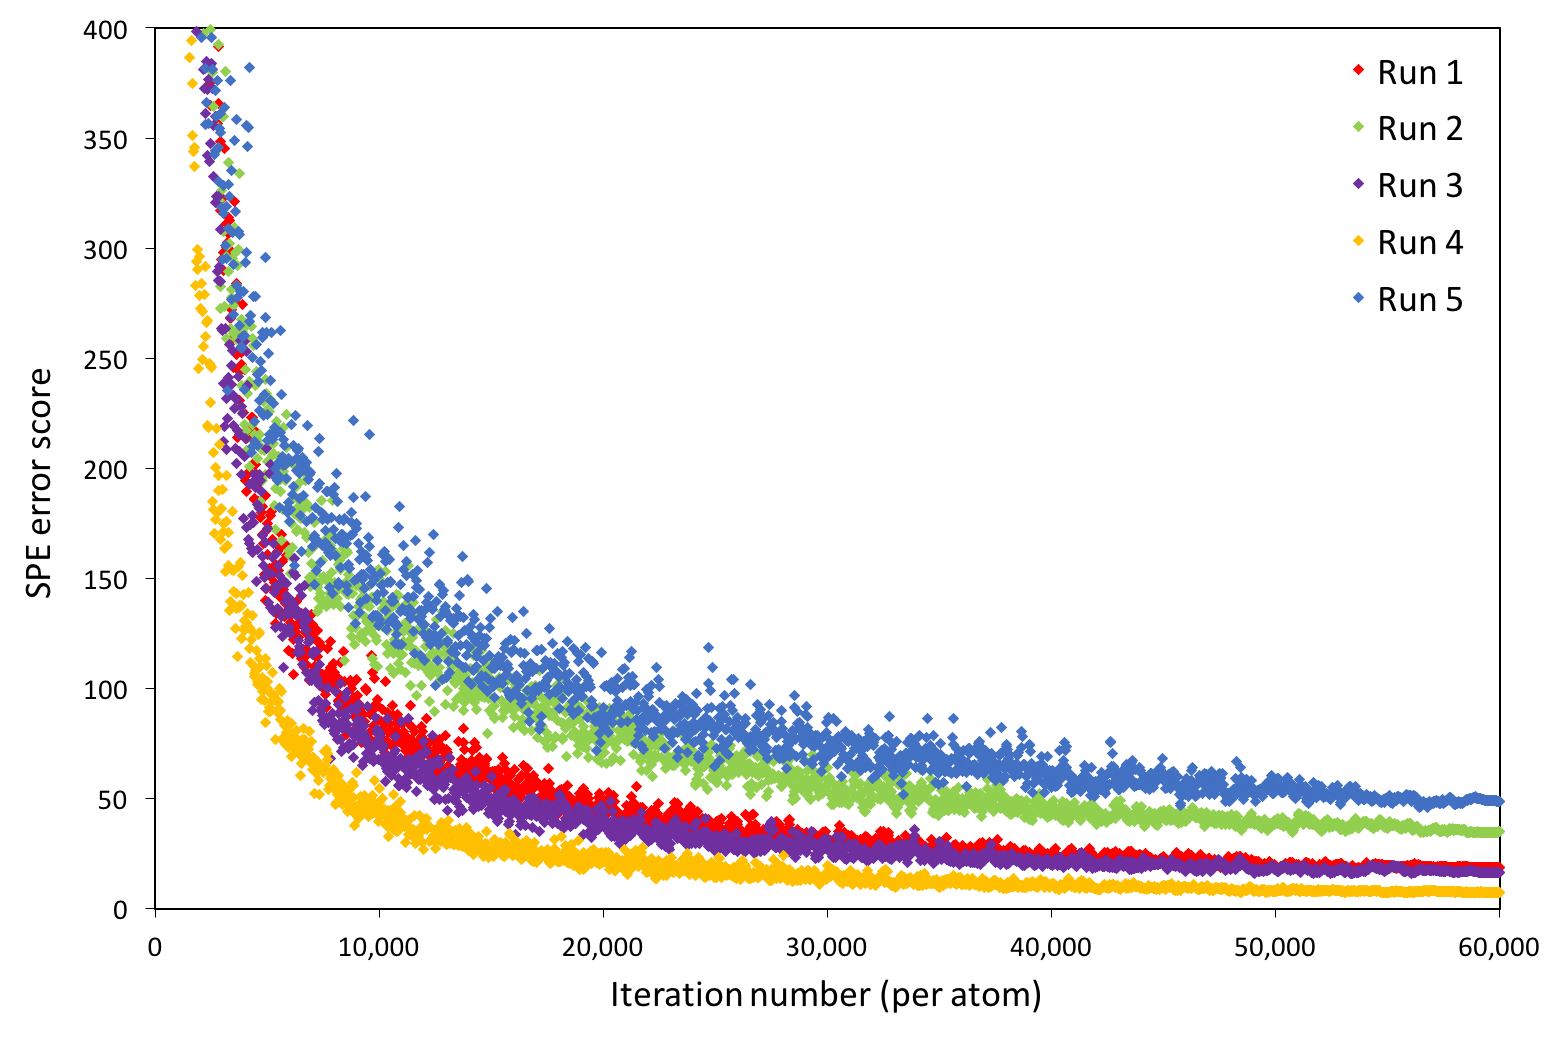
\includegraphics[width=\textwidth]{figures/spe_convergence/spe_convergence}

\caption{The SPE error score, a measure of how many distance constraints are violated, shown over the course of 5 separate runs on CDK2.
Initially the random atomic coordinates give a high score.
As the iterative procedure occurs atoms that violate distance constraints are moved, reducing the SPE error score.}

\label{fig:spe_convergence}
\end{figure}


Figure~\ref{fig:score_procheck} shows the final SPE error score for each structure generated in the CDK2 ensemble plotted against the PROCHECK overall G-factor.
It can be seen that most structures have an overall G-factor between -0.4 and -0.6, and that there is an inverse correlation between overall G-factor and SPE error score.
This is to be expected as structures which have more violations of the distance constraints are more likely to have poor stereochemical quality.


\begin{figure}
\centering

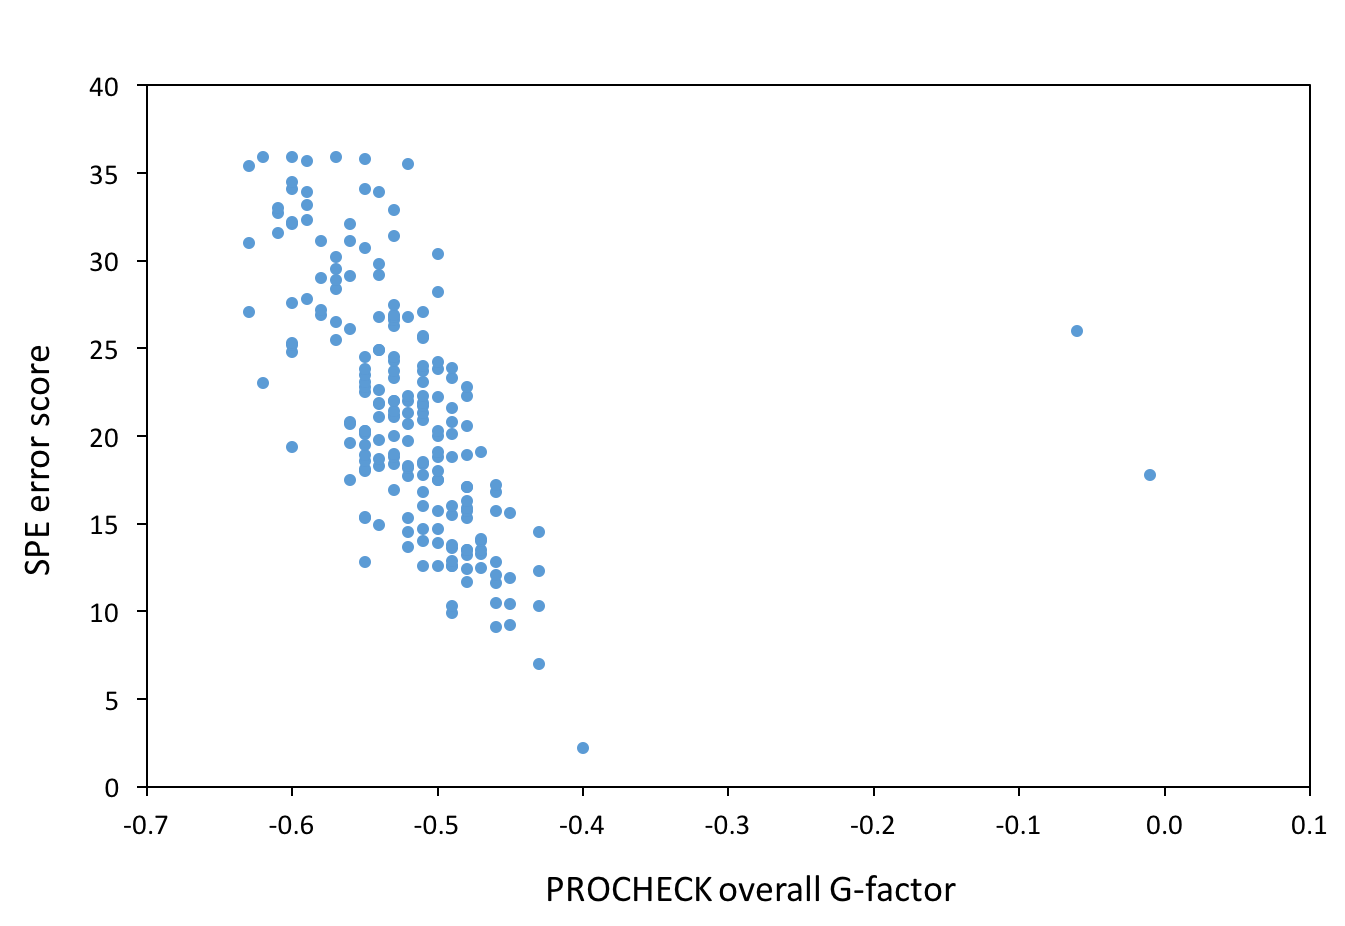
\includegraphics[width=\textwidth]{figures/score_procheck/score_procheck}

\caption{The SPE error score of each structure in the CDK2 ensemble is plotted against the PROCHECK overall G-factor of the structure.
Note that an ensemble of 300 structures was generated and only the 200 structures with the lowest SPE error score were retained (see Methods section).}

\label{fig:score_procheck}
\end{figure}


\subsubsection{Apo/holo dataset}

In order to examine the ability of existing non-MD methods to generate ensembles that span conformational changes, a dataset of apo (no modulator) and holo (modulator bound) structures was used \cite{Atilgan2010}.
The proteins have RMSD between apo and holo structures ranging from 2 \AA\ to 19 \AA, and represent a variety of domain, subdomain and subunit motions.
tCONCOORD \cite{Seeliger2007} and NMSim \cite{Kruger2012} both seek to model conformational changes such as those in the dataset.
Default parameters were used to produce 250 structures for each protein from tCONCOORD and NMSim.
The lowest RMSD of the structures in an ensemble to a particular crystal structure was taken as a measure of how close the ensemble came to exploring the conformational space of that crystal structure.
This can be seen in Table~\ref{tab:ensemble_dataset}.

When the apo structure is used as input, structures similar to the apo structure are generated by both methods.
The median lowest RMSD to the apo crystal is 1.44 \AA\ for tCONCOORD and 0.71 \AA\ for NMSim.
However, structures similar to the holo crystal are not sampled.
The median lowest RMSD to the holo crystal is 4.15 \AA\ for tCONCOORD and 4.68 \AA\ for NMSim.
In a similar manner, when the holo structure is used as input to tCONCOORD and NMSim the ensembles sample the holo structure but not the apo structure.

ExProSE, as expected because it uses both the apo and holo crystals as input, is able to generate structures close to both crystals - see Table~\ref{tab:ensemble_dataset_ex}.
For 11 out of the 12 proteins ExProSE can generate a structure closer to the holo crystal than the other methods, where the other methods use the apo structure as input.
For the opposite case, comparing to the apo crystal, ExProSE also generates a closer structure for 11 out of 12 proteins.
Hence ExProSE is useful for generating ensembles when two or more structures are available.

The median PROCHECK overall G-factor across all generated structures is -0.99 for ExProSE, indicating that PROCHECK produces structures that are generally acceptable.
The values for NMSim and tCONCOORD are -0.32 and -1.83 respectively, indicating that NMSim produces good quality structures and tCONCOORD produces structures with poor stereochemical quality.
The stereochemistry of generated structures can be improved by energy minimisation (see below).


\begin{sidewaystable}
\centering

\begin{small}
% Table generated by Excel2LaTeX from sheet 'methods'
\begin{tabular}{rrrrrllllllll}
\hline
      &       &       &       &       & \multicolumn{2}{c}{\textbf{tCONCOORD}} & \multicolumn{2}{c}{\textbf{tCONCOORD}} & \multicolumn{2}{c}{\textbf{NMSim}} & \multicolumn{2}{c}{\textbf{NMSim}} \\
      &       &       &       &       & \multicolumn{2}{c}{\textbf{from apo}} & \multicolumn{2}{c}{\textbf{from holo}} & \multicolumn{2}{c}{\textbf{from apo}} & \multicolumn{2}{c}{\textbf{from holo}} \\
      &       &       &       &       & \multicolumn{8}{c}{Lowest RMSD from 250 generated structures to apo/holo crystal / \AA} \\
\multicolumn{1}{l}{\textbf{Protein name}} & \multicolumn{1}{l}{\textbf{Apo PDB}} & \multicolumn{1}{l}{\textbf{Holo PDB}} & \multicolumn{1}{l}{\textbf{RMSD / \AA}} & \multicolumn{1}{l}{\textit{\textbf{N}}} & \textbf{Apo} & \textbf{Holo} & \textbf{Apo} & \textbf{Holo} & \textbf{Apo} & \textbf{Holo} & \textbf{Apo} & \textbf{Holo} \\
\hline
\multicolumn{1}{l}{OxyR transcription factor} & \multicolumn{1}{l}{1I6A} & \multicolumn{1}{l}{1I69} & \multicolumn{1}{l}{2.44} & \multicolumn{1}{l}{206} & 1.18  & 2.69  & 2.66  & 1.12  & 1.04  & 2.61  & 2.51  & 0.72 \\
\multicolumn{1}{l}{Ferric binding protein}    & \multicolumn{1}{l}{1D9V} & \multicolumn{1}{l}{1MRP} & \multicolumn{1}{l}{2.68} & \multicolumn{1}{l}{309} & 1.22  & 1.81  & 1.88  & 1.41  & 0.62  & 2.07  & 2.31  & 0.71 \\
\multicolumn{1}{l}{Aspartate receptor}        & \multicolumn{1}{l}{1LIH} & \multicolumn{1}{l}{2LIG} & \multicolumn{1}{l}{2.77} & \multicolumn{1}{l}{157} & 1.16  & 2.73  & 2.94  & 1.48  & 0.94  & 2.45  & 2.65  & 0.80 \\
\multicolumn{1}{l}{HIV-1 rev. transcriptase}  & \multicolumn{1}{l}{2HMI} & \multicolumn{1}{l}{3HVT} & \multicolumn{1}{l}{3.81} & \multicolumn{1}{l}{555} & 2.49  & 4.11  & 4.66  & 3.44  & 0.64  & 3.28  & 3.14  & 0.78 \\
\multicolumn{1}{l}{Maltose binding protein}   & \multicolumn{1}{l}{1OMP} & \multicolumn{1}{l}{3MBP} & \multicolumn{1}{l}{3.88} & \multicolumn{1}{l}{370} & 0.97  & 2.62  & 2.66  & 0.89  & 0.71  & 2.35  & 2.39  & 0.57 \\
\multicolumn{1}{l}{Small G protein Arf6}      & \multicolumn{1}{l}{1E0S} & \multicolumn{1}{l}{2J5X} & \multicolumn{1}{l}{4.44} & \multicolumn{1}{l}{164} & 0.99  & 4.18  & 4.23  & 0.96  & 0.66  & 4.00  & 4.23  & 0.86 \\
\multicolumn{1}{l}{Immunoglobulin}            & \multicolumn{1}{l}{1MCP} & \multicolumn{1}{l}{4FAB} & \multicolumn{1}{l}{5.95} & \multicolumn{1}{l}{214} & 1.65  & 3.60  & 3.80  & 1.51  & 0.62  & 5.35  & 3.63  & 0.79 \\
\multicolumn{1}{l}{Myosin}                    & \multicolumn{1}{l}{1VOM} & \multicolumn{1}{l}{2AKA} & \multicolumn{1}{l}{6.23} & \multicolumn{1}{l}{730} & 2.60  & 5.11  & 5.63  & 2.38  & 0.73  & 5.53  & 5.77  & 0.63 \\
\multicolumn{1}{l}{Adenylate kinase}          & \multicolumn{1}{l}{4AKE} & \multicolumn{1}{l}{1AKE} & \multicolumn{1}{l}{7.19} & \multicolumn{1}{l}{214} & 1.70  & 4.88  & 6.00  & 1.18  & 0.58  & 6.16  & 6.09  & 0.74 \\
\multicolumn{1}{l}{Serpin}                    & \multicolumn{1}{l}{1PSI} & \multicolumn{1}{l}{7API} & \multicolumn{1}{l}{8.96} & \multicolumn{1}{l}{372} & 1.20  & 8.71  & 8.93  & 1.51  & 0.71  & 8.22  & 8.97  & 0.97 \\
\multicolumn{1}{l}{GroEL}                     & \multicolumn{1}{l}{1AON} & \multicolumn{1}{l}{1OEL} & \multicolumn{1}{l}{12.6} & \multicolumn{1}{l}{524} & 3.01  & 9.72  & 9.61  & 2.45  & 0.87  & 10.8  & 10.1  & 0.48 \\
\multicolumn{1}{l}{Topoisomerase II}          & \multicolumn{1}{l}{1BGW} & \multicolumn{1}{l}{1BJT} & \multicolumn{1}{l}{18.8} & \multicolumn{1}{l}{664} & 3.36  & 17.5  & 17.0  & 3.34  & 0.81  & 18.0  & 17.3  & 0.65 \\
\hline
\multicolumn{5}{r}{\textbf{Median across all proteins}} & 1.44  & 4.15  & 4.45  & 1.50  & 0.71  & 4.68  & 3.93  & 0.73 \\
\hline
\end{tabular}
\end{small}

\caption{Comparison of ensemble generation methods.
The columns Apo PDB and Holo PDB refer to the PDB IDs of the apo and holo structures used.
RMSD is the all-atom RMSD in \AA\ between the apo and holo structures.
The rows are ordered by increasing RMSD.
\textit{N} is the number of residues in common between the apo and holo chains used.
The values on the right are the lowest RMSD in \AA\ of the structures in an ensemble produced using the method and input indicated, to the crystal structure indicated.
A low value indicates that the ensemble sampled a structure close to the crystal structure.
The median of the lowest RMSDs for each method/input combination is also given.}

\label{tab:ensemble_dataset}
\end{sidewaystable}


\begin{table}
\centering

\begin{small}
% Table generated by Excel2LaTeX from sheet 'exprose'
\begin{tabular}{rrrrrll}
\hline
      &       &       &       &       & \multicolumn{2}{c}{Lowest RMSD from 250 generated ExProSE structures to apo/holo crystal / \AA} \\
\multicolumn{1}{l}{\textbf{Protein name}} & \multicolumn{1}{l}{\textbf{Apo PDB}} & \multicolumn{1}{l}{\textbf{Holo PDB}} & \multicolumn{1}{l}{\textbf{RMSD / \AA}} & \multicolumn{1}{l}{\textit{\textbf{N}}} & \textbf{Apo} & \textbf{Holo} \\
\hline
\multicolumn{1}{l}{OxyR transcription factor} & \multicolumn{1}{l}{1I6A} & \multicolumn{1}{l}{1I69} & \multicolumn{1}{l}{2.44} & \multicolumn{1}{l}{206} & 1.02  & 1.16 \\
\multicolumn{1}{l}{Ferric binding protein}    & \multicolumn{1}{l}{1D9V} & \multicolumn{1}{l}{1MRP} & \multicolumn{1}{l}{2.68} & \multicolumn{1}{l}{309} & 0.90  & 1.08 \\
\multicolumn{1}{l}{Aspartate receptor}        & \multicolumn{1}{l}{1LIH} & \multicolumn{1}{l}{2LIG} & \multicolumn{1}{l}{2.77} & \multicolumn{1}{l}{157} & 1.25  & 0.88 \\
\multicolumn{1}{l}{HIV-1 rev. transcriptase}  & \multicolumn{1}{l}{2HMI} & \multicolumn{1}{l}{3HVT} & \multicolumn{1}{l}{3.81} & \multicolumn{1}{l}{555} & 1.84  & 1.45 \\
\multicolumn{1}{l}{Maltose binding protein}   & \multicolumn{1}{l}{1OMP} & \multicolumn{1}{l}{3MBP} & \multicolumn{1}{l}{3.88} & \multicolumn{1}{l}{370} & 0.85  & 1.50 \\
\multicolumn{1}{l}{Small G protein Arf6}      & \multicolumn{1}{l}{1E0S} & \multicolumn{1}{l}{2J5X} & \multicolumn{1}{l}{4.44} & \multicolumn{1}{l}{164} & 1.70  & 1.88 \\
\multicolumn{1}{l}{Immunoglobulin}            & \multicolumn{1}{l}{1MCP} & \multicolumn{1}{l}{4FAB} & \multicolumn{1}{l}{5.95} & \multicolumn{1}{l}{214} & 3.90  & 5.33 \\
\multicolumn{1}{l}{Myosin}                    & \multicolumn{1}{l}{1VOM} & \multicolumn{1}{l}{2AKA} & \multicolumn{1}{l}{6.23} & \multicolumn{1}{l}{730} & 2.38  & 1.89 \\
\multicolumn{1}{l}{Adenylate kinase}          & \multicolumn{1}{l}{4AKE} & \multicolumn{1}{l}{1AKE} & \multicolumn{1}{l}{7.19} & \multicolumn{1}{l}{214} & 3.15  & 1.98 \\
\multicolumn{1}{l}{Serpin}                    & \multicolumn{1}{l}{1PSI} & \multicolumn{1}{l}{7API} & \multicolumn{1}{l}{8.96} & \multicolumn{1}{l}{372} & 1.08  & 1.01 \\
\multicolumn{1}{l}{GroEL}                     & \multicolumn{1}{l}{1AON} & \multicolumn{1}{l}{1OEL} & \multicolumn{1}{l}{12.6} & \multicolumn{1}{l}{524} & 3.13  & 3.70 \\
\multicolumn{1}{l}{Topoisomerase II}          & \multicolumn{1}{l}{1BGW} & \multicolumn{1}{l}{1BJT} & \multicolumn{1}{l}{18.8} & \multicolumn{1}{l}{664} & 3.54  & 5.10 \\
\hline
\multicolumn{5}{r}{\textbf{Median across all proteins}} & 1.77  & 1.69 \\
\hline
\end{tabular}
\end{small}


\caption{Ability of ExProSE ensembles to reach apo and holo structures.
The columns Apo PDB, Holo PDB, RMSD and \textit{N} are the same as in Table~\ref{tab:ensemble_dataset}.
The values on the right are the lowest RMSD in \AA\ of the structures in an ExProSE ensemble to the crystal structure indicated.
A low value indicates that the ensemble sampled a structure close to the crystal structure.
The median of the lowest RMSDs is also given.}

\label{tab:ensemble_dataset_ex}
\end{table}


\subsubsection{T4-lysozyme}

Here, we demonstrate that ExProSE can generate structures close to crystals not used as input.
Lysozymes damage bacterial cell walls by catalysing the hydrolysis of peptidoglycans.
Bacteriophage T4-lysozyme is a suitable protein for analysing conformational variability as there are many crystal structures available and MD simulations of the protein have shown that simulations up to 200 ns do not reliably reach both the open and closed conformations \cite{Seeliger2007}.
The pairwise RMSDs of the crystals range from 0.64 \AA\ to 4.25 \AA.

An ensemble was generated using ExProSE from the open (PDB ID 169L, chain E) and closed (PDB ID 2LZM) conformations.
Four random structures from this ensemble are shown compared to the open and closed crystal structures in Figure~\ref{fig:t4l}A.
Principal components analysis (PCA) can be carried out on an ensemble of structures to find the orthogonal motions that describe the variation in the ensemble.
Figure~\ref{fig:t4l}B shows the projections of the generated ensemble and the 38 crystal structures used in a prior study \cite{DeGroot1998} onto the first and second principal components (PCs), which account for 70\% and 12\% of the motion respectively.
The dominant first eigenvector corresponds to opening and closing of the structure.
It can be seen that the method is able to sample conformations corresponding to experimentally-observed structures, as the ensembles largely overlap.

Ensembles produced by tCONCOORD starting from the open and closed structures separately are shown in Figure~\ref{fig:t4l}C.
As demonstrated previously on other proteins, the ensemble generated from the open structure cannot reach all the way to the closed structure, and vice versa.
The tCONCOORD ensembles also sample structures not found in the ensemble of crystal structures, particularly when using the open conformation as input.
This tendency of tCONCOORD to produce ensembles with too much structural variability was also noted by the authors \cite{Seeliger2009}.

Ensembles produced by NMSim starting from the open and closed structures separately are shown in Figure~\ref{fig:t4l}D.
In this case, the ensemble generated from the open and closed structures can largely span the conformational space.
Similar to tCONCOORD, regions not explored by the crystals are sampled by NMSim.
For example, there is one model in the ensemble generated from the open structure that has an RMSD of 7.38 \AA\ to the nearest crystal structure.

Alternative parameters were also used for tCONCOORD and NMSim to see how the ensembles varied - see Figure~\ref{fig:method_params}.
For tCONCOORD decreasing the upper bound for long range constraints, and/or turning off close pairs as constraints, had little effect on the distribution of the ensembles.
For NMSim using the parameters for small scale motions led to ensembles that could not span the conformational space.
In each case the default parameters gave similar or better coverage of the conformational space of the crystals by visual inspection, and were hence used for the analysis below.


\begin{figure}
\centering

%\includegraphics[width=\textwidth]{figures/t4l}
% Make this figure bigger with large ensemble in PyMol

\caption{T4-lysozyme ensembles.
(\textbf{A}) Four structures generated from ExProSE using the open (PDB ID 169L, chain E)  and closed (PDB ID 2LZM) conformations as input are shown in orange.
The crystal structures of the open and closed conformations are shown in blue and green respectively for reference.
The arrow shows the opening motion caused by the breaking of a hydrogen bond between ARG137 and GLU22.
(\textbf{B}) Projections of the 38 crystal structures used in a prior study \cite{DeGroot1998} onto the first (x-axis) and second (y-axis) PCs of the PCA of the crystal structures, which account for 70\% and 12\% of the motion respectively (black dots).
Projections from the ensembles generated with ExProSE are also shown (red dots).
(\textbf{C}) Projections of two tCONCOORD ensembles on the same plot as (B).
An ensemble using the open structure as input (blue dots) and an ensemble using the closed structure as input (yellow dots) are shown.
(\textbf{D}) Projections of two NMSim ensembles with parameters for large scale motions on the same plot as (B).
An ensemble using the open structure as input (blue dots) and an ensemble using the closed structure as input (yellow dots) are shown.
Figure based on Figure~1 from Greener and Sternberg 2017 \cite{Greener2017}.}

\label{fig:t4l}
\end{figure}


\begin{figure}
\centering

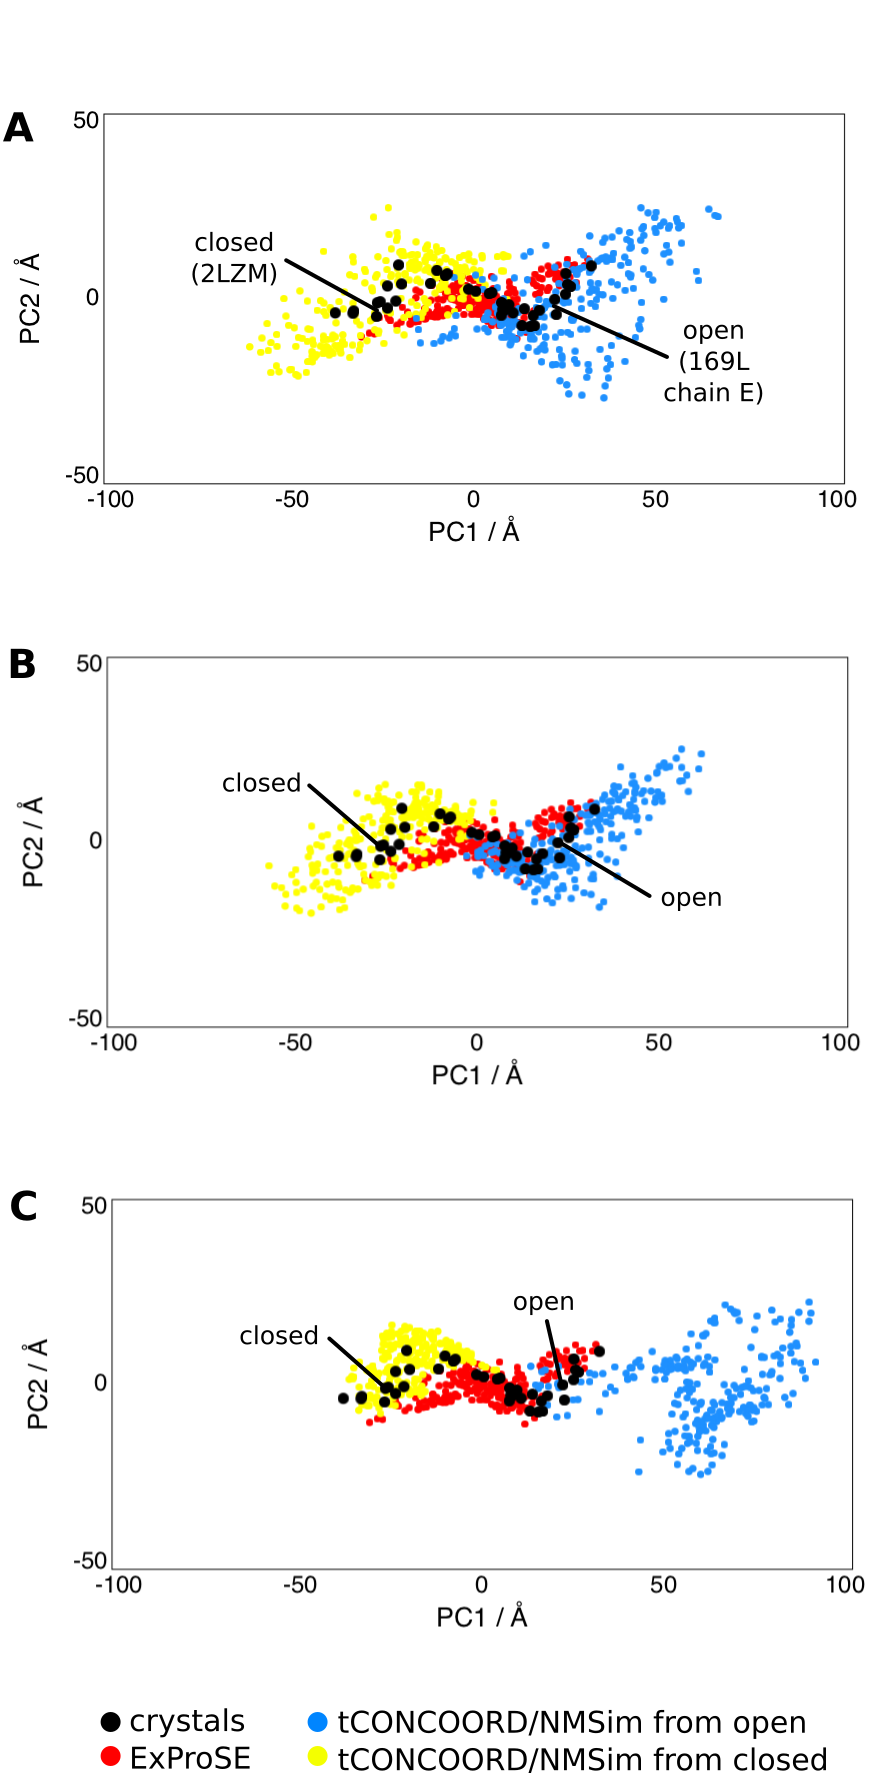
\includegraphics[width=0.55\textwidth]{figures/method_params/method_params}

\caption{Ensemble generation for T4-lysozyme with different parameters.
Projections of tCONCOORD/NMSim ensembles from the open (blue dots) and closed (yellow dots) structures onto the PCA of the crystal structures are shown.
Similar to Figure~\ref{fig:t4l}, in each graph the projections of the crystals (black dots) and projections from the ensembles generated with ExProSE (red dots) are also shown.
(A) tCONCOORD ensembles with the upper bound for long range constraints set to 1.3 \AA\ (default 2.0 \AA ).
(B) tCONCOORD ensembles with the upper bound for long range constraints set to 1.3 \AA\ and close pairs not used as constraints.
(C) NMSim ensembles using the default parameters for small scale motions.
Figure based on Figure~S1 from Greener and Sternberg 2017 \cite{Greener2017}.}

\label{fig:method_params}
\end{figure}


T4-lysozyme was also studied with MD.
50 ns MD runs starting from the closed conformation were not able to reach the open conformation and vice versa - see Figure~\ref{fig:t4l_md}A and \ref{fig:t4l_md}B.
Targeted MD runs starting from the closed conformation and targeting the open conformation (and vice versa) were also carried out.
In targeted MD the atoms are guided to a target structure with the use of a steering force that seeks to minimise the RMSD of the structure to the target structure.
These ensembles can be seen in Figure~\ref{fig:t4l_md}C and \ref{fig:t4l_md}D, and are generally able to cross conformational space over the course of around 20 ns.
However beyond this time they show unpredictable behaviour and can deviate from the experimental structures.
Retaining only the structures up to 20 ns, as in Figure~\ref{fig:t4l_md}C and \ref{fig:t4l_md}D, gives ensembles that largely overlap with the experimental structures.


\begin{figure}
\centering

\includegraphics[width=0.5\textwidth]{figures/t4l_md/t4l_md}

\caption{MD T4-lysozyme ensembles.
Projections of two repeats of a particular MD run onto the PCA of the crystal structures are shown (blue and yellow dots), with snapshots taken every 100 ps.
Similar to Figure~\ref{fig:t4l}, in each graph the projections of the crystals are also shown (black dots).
(\textbf{A}) 50 ns MD runs starting from the closed structure (PDB ID 2LZM).
(\textbf{B}) 50 ns MD runs starting from the open structure (PDB ID 169L).
(\textbf{C}) 20 ns targeted MD runs starting from the closed structure and targeting the open structure.
(\textbf{D}) 20 ns targeted MD runs starting from the open structure and targeting the closed structure.
Figure based on Figure~2 from Greener and Sternberg 2017 \cite{Greener2017}.}

\label{fig:t4l_md}
\end{figure}


By combining tCONCOORD, NMSim and targeted MD ensembles generated using the open and closed structures as input, a fair comparison to ExProSE can be made.
A generated ensemble should ideally contain models close to all the crystal structures.
The degree to which this occurs for ExProSE ensembles, and combined ensembles for tCONCOORD, NMSim and targeted MD up to 20 ns, is shown in Figure~\ref{fig:t4l_rmsd}A.
It can be seen that ExProSE is able to generate structures close to all crystals, with all crystals having an RMSD of 1.7 \AA\ or less to a generated structure.
For 26 out of 38 crystals ExProSE generates a model closer to the crystal than NMSim.
It generates a closer model than tCONCOORD in all cases.
For 15 out of 38 crystals ExProSE generates a model closer to the crystal than targeted MD.
However, this is the case for 14 out of the 27 structures that have an RMSD of more than 1.0 \AA\ to both the open and closed reference structures.
Of these 27, ExProSE performs better for all of the 4 structures that have an RMSD of more than 1.5 \AA.
Hence ExProSE is able to generate better models than the other methods for crystals which are far from either input structure, as seen on the right side of Figure~\ref{fig:t4l_rmsd}A.
The PROCHECK overall G-factor of the closest models for each method is shown in Figure~\ref{fig:t4l_rmsd}B.
ExProSE is able to produce models of acceptable quality close to all the crystals, even for those further from the input structures.

In order to determine whether the stereochemical quality of generated structures could be improved, energy minimisation was carried out on all structures.
For all methods, energy minimisation improved median PROCHECK overall G-factors.
Across the ensembles the median values increased from the range [-2.23, -0.45] to the range [-0.31, -0.17] - see Table~\ref{tab:energy_minimisation}.
This shows that stereochemical problems in generated structures can in general be improved by energy minimisation, important if using generated structures for docking studies.

By using two input structures rather than one, ExProSE is able to produce models of acceptable quality close to other crystal structures.
It can explore conformational space better than methods that use a single structure as input.


\begin{figure}
\centering

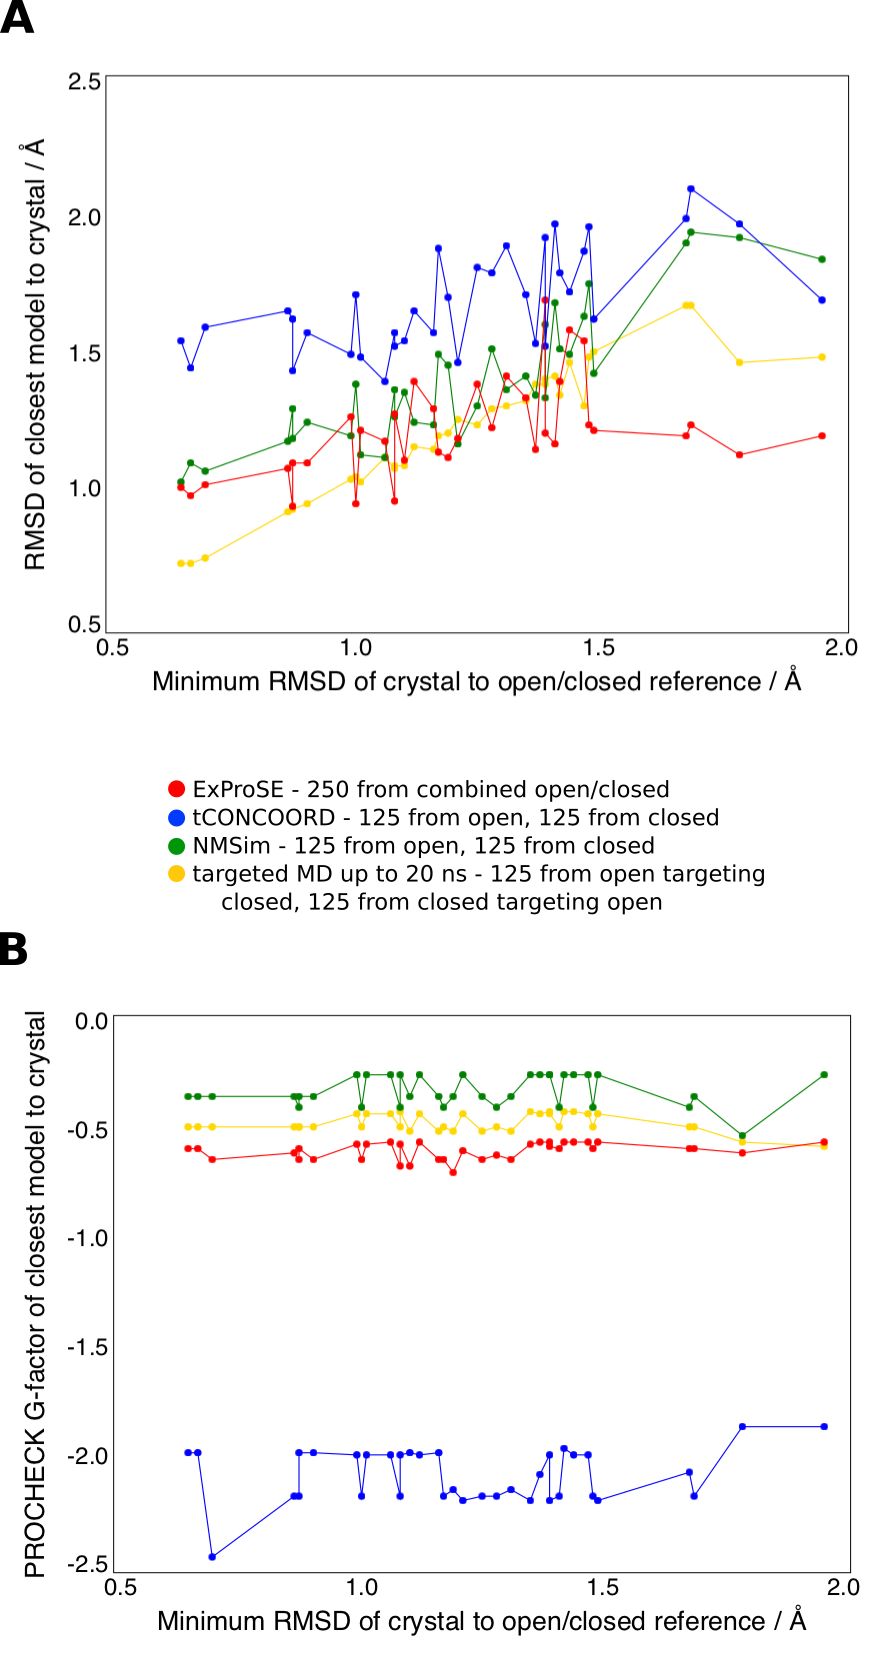
\includegraphics[width=0.6\textwidth]{figures/t4l_rmsd/t4l_rmsd}

\caption{Closest models from each ensemble to T4-lysozyme crystal structures.
(\textbf{A}) The RMSD of the closest model from each generated ensemble to the crystal structures.
The crystal structures are sorted by the lower of the two RMSD values to the open and closed crystals used as input.
The crystals used as inputs are omitted from the graph.
(\textbf{B}) PROCHECK overall G-factors of the closest model from each generated ensemble to the crystal structures.
The crystal structures are sorted as in (A).
Figure based on Figure~3 from Greener and Sternberg 2017 \cite{Greener2017}.}

\label{fig:t4l_rmsd}
\end{figure}


\begin{table}
\centering

\begin{scriptsize}
% Table generated by Excel2LaTeX from sheet 'minimise'
\begin{tabular}{ l l p{4cm} p{4cm} }
\hline
\textbf{Method} & \textbf{Strucure(s) used} & \textbf{Median overall G-factor\newline before energy minimisation} & \textbf{Median overall G-factor\newline after energy minimisation} \\
\hline
ExProSE     & open and closed                 & -0.58 & -0.26 \\
tCONCOORD   & open                            & -2.23 & -0.31 \\
tCONCOORD   & closed                          & -2.09 & -0.27 \\
NMSim       & open                            & -0.50 & -0.31 \\
NMSim       & closed                          & -0.45 & -0.29 \\
targeted MD & starting open, targeting closed & -0.56 & -0.17 \\
targeted MD & starting closed, targeting open & -0.57 & -0.20 \\
\hline
\end{tabular}
\end{scriptsize}

\caption{Improvement in stereochemical quality on energy minimisation.
The structures in each ensemble were analysed with PROCHECK and the median overall G-factor across the ensemble was noted.
The median of the overall G-factor of each structure after energy minimisation was also recorded.}

\label{tab:energy_minimisation}
\end{table}


\subsection{Ensemble perturbation for CDK2}

Here, we demonstrate that ExProSE ensembles can be perturbed to reveal modulating sites.
CDK2 is a protein kinase essential for the G1/S phase transition in the cell cycle - see (section ref).
An ExProSE ensemble was generated using the apo native structure (PDB ID 1HCL) and the holo structure bound to two ANS molecules in an allosteric site (PDB ID 3PXF).
The ANS-bound structure is inactive, as ANS binding causes a conformational shift in the C-helix that prevents cyclin binding \cite{Betzi2011}.
A further screening study has found potential modulators for the ANS binding site \cite{Rastelli2014}.

Figure~\ref{fig:cdk}A shows the pockets predicted by LIGSITE\textsuperscript{\it cs} \cite{Huang2006} on CDK2 bound to two ANS molecules.
The ensemble perturbation procedure was carried out at each of the 8 pocket centres as described in the experimental procedures.
In brief, additional constraints are added representing a modulator bound in the selected pocket.
Projections of the structures of the unperturbed ensemble and the structures of the ensemble with perturbation at the pocket centre are shown in Figure~\ref{fig:cdk}B, one graph per pocket centre.
The third PC was chosen for visualisation instead of the second as it represents the inactivating motion of the C-helix, whereas the second PC represents a rotation in the region of the protein considered to be functionally less important, the C-lobe.

% This should link to later
Site 1 in Figure~\ref{fig:cdk}A and \ref{fig:cdk}B is the ANS allosteric pocket.
Simulating a modulator there shifts the ensemble towards the inactive state, agreeing with previous experimental data \cite{Betzi2011}.
Site 2 is the ATP-binding site and there is no change in the ensemble by simulating a modulator there.
This is encouraging as ATP binding does not cause structural changes that lead to cyclin dissociation.
Site 3 is found in a pocket near the activation segment.
A shift in the ensemble towards the inactive state is seen on perturbation at this site.
In fact this site is close to a potential allosteric site suggested in another computational study \cite{Pitt2014}, and is part of the region associated with cyclin-binding.
This indicates that the site could potentially be an allosteric site, though further effort would be required to determine whether it is druggable.
Simulating modulators at sites 4 to 8 does not shift the ensemble, suggesting that binding at these sites is unable to cause an allosteric effect.
No allosteric modulators have been reported experimentally for these sites.


\begin{figure}
\centering

%\includegraphics[width=\textwidth]{figures/cdk}

\caption{CDK2 pockets and projections of ensembles.
(\textbf{A}) CDK2 in its holo conformation bound to two ANS molecules in the allosteric site (PDB ID 3PXF).
CDK2 is shown as a green cartoon with the two bound ANS shown as blue sticks.
Pocket centres predicted by LIGSITE\textsuperscript{\it cs} are shown as purple spheres.
The pockets are numbered by descending volume.
Pocket 1 represents the ANS allosteric pocket.
Pocket 2 represents the ATP binding pocket.
(\textbf{B}) Structures generated using ExProSE, with input structures the apo and holo structures (PDB ID 1HCL and 3PXF respectively), are shown as red dots.
The axes are projections onto the first (x-axis) and third (y-axis) PCs of the ExProSE ensemble, which account for 35\% and 8\% of the motion respectively.
The blue dots represent the structures in the ensemble with perturbation at pocket centres 1-8 from (A).}

\label{fig:cdk}
\end{figure}


\subsection{Allosteric site prediction}

Systematic methods to predict allosteric sites on proteins are necessary to utilise the potential advantages of allosteric drugs.
A diverse dataset of 58 apo/holo pairs representing the unbound protein and the protein bound to a known allosteric modulator was assembled from the ASD \cite{Shen2016}.
This dataset showed a large range in protein size (153 to 955 residues) and included a variety of proteins including transcriptional regulators, transporters and protein kinases.

LIGSITE\textsuperscript{\it cs} was used to predict pockets on the holo crystal structures and ExProSE was used to generate a perturbed ensemble for each pocket centre as described in the experimental procedures.
These perturbed ensembles were used to rank the pockets in terms of predicted allosteric effect.
In this study a correct prediction for a protein indicates that an allosteric pocket was ranked first or second.
This criterion was chosen as a measure of success because typically the top few pockets predicted by a method would be examined and studied further.

The ability of ExProSE to predict allosteric pockets on the dataset is compared to existing allosteric prediction methods, which are run with the holo crystal structures as input.
This was found to give better results for the existing methods than using the apo crystals.
PARS \cite{Panjkovich2014} uses NMA with and without a predicted modulator to predict changes in flexibility.
STRESS \cite{Clarke2016} is an implementation of the earlier binding leverage algorithm \cite{Mitternacht2011}, which models how perturbations due to binding couple to the motions of the protein as expressed by low-frequency normal modes.
AlloPred \cite{Greener2015} uses perturbation of normal modes and pocket features in a machine learning approach to predict allosteric pockets.
It should be noted that different criteria are used to define an allosteric pocket for each method, due to the nature of their output - see the experimental procedures.
For 27 of 58 proteins ExProSE ranked an allosteric pocket first or second, performing better than the other three methods.
This is shown in Table~\ref{tab:allosteric_methods}.
Only 7 proteins have an allosteric pocket ranked first or second by all four methods.
In 3 cases ExProSE makes a correct prediction for a protein while none of the other methods did.

The performance of the allosteric prediction methods is also compared to the pocket prediction methods LIGSITE\textsuperscript{\it cs} and Fpocket \cite{LeGuilloux2009} in Table~\ref{tab:allosteric_methods}.
LIGSITE\textsuperscript{\it cs} and Fpocket are effective at finding allosteric sites, both ranking an allosteric pocket first or second for 31 out of 58 proteins, even though they are not designed specifically for allosteric site prediction.
This is not too surprising as the holo structures were used as input, so the modulator had a reasonable chance of being in one of the two largest pockets.
However ExProSE is still valuable as it finds smaller, less obvious allosteric pockets.
This could be due to the extra structural information used as input.
For example, ExProSE in 6 cases finds sites not ranked in the top 2 by LIGSITE\textsuperscript{\it cs} and in 8 cases finds sites not ranked in the top 2 by Fpocket.
ExProSE shows the best complementarity to the pocket prediction methods along with STRESS, which makes fewer correct predictions.
ExProSE also gives information on how the ensemble may be affected by the modulators, as demonstrated in Figure~\ref{fig:cdk}, allowing inspection of the predicted structural and dynamic changes arising from perturbation.

The performance on each protein by each method is shown in Table~\ref{tab:allosteric_proteins}.
This is to our knowledge the first systematic comparison of multiple allosteric prediction methods.
49 of 58 proteins had an allosteric pocket ranked first or second by at least one of the 6 methods compared in Table~\ref{tab:allosteric_methods}.
This complementarity indicates the potential for a meta approach that combines predictions from multiple methods.


\begin{table}
\centering

% Table generated by Excel2LaTeX from sheet 'summary'
\begin{tabular}{ p{3cm} p{3cm} p{3cm} p{3cm} }
\hline
\textbf{Method} & \textbf{Correct in top 2\newline (out of 58)} & \textbf{Unique from\newline LIGSITE\textsuperscript{\it cs}} & \textbf{Unique from\newline Fpocket} \\
\hline
ExProSE                         & 27 & 6/27 & 8/27 \\
PARS                            & 25 & 3/25 & 7/25 \\
STRESS                          & 18 & 6/18 & 8/18 \\
AlloPred                        & 26 & 5/26 & 1/26 \\
LIGSITE\textsuperscript{\it cs} & 31 & -    & 8/31 \\
Fpocket                         & 31 & 8/31 & -    \\
\hline
\end{tabular}

\caption{Performance of allosteric site prediction methods on a dataset of 58 known allosteric proteins.
Correct in top 2 is the number of proteins for which the method successfully ranked an allosteric pocket first or second.
The definition for an allosteric pocket is given in the experimental procedures.
The number of correct predictions by each method that are unique from the correct predictions of LIGSITE\textsuperscript{\it cs} and Fpocket is also shown.
STRESS could not run on 4 proteins as they were too small.}

\label{tab:allosteric_methods}
\end{table}


\begin{table}
\centering

\begin{scriptsize}
% Table generated by Excel2LaTeX from sheet 'full'
\begin{tabular}{rrrrrrrrrrrr}
\hline
\multicolumn{1}{r}{\textbf{Protein name}} & \multicolumn{1}{l}{\textbf{Apo PDB}} & \multicolumn{1}{l}{\textbf{Holo PDB}} & \multicolumn{1}{l}{\textbf{Apo chains}} & \multicolumn{1}{l}{\textbf{Holo chains}} & \multicolumn{1}{l}{\textbf{N}} & \multicolumn{1}{l}{\begin{sideways}\textbf{ExProSE}\end{sideways}} & \multicolumn{1}{l}{\begin{sideways}\textbf{PARS}\end{sideways}} & \multicolumn{1}{l}{\begin{sideways}\textbf{STRESS}\end{sideways}} & \multicolumn{1}{l}{\begin{sideways}\textbf{AlloPred}\end{sideways}} & \multicolumn{1}{l}{\begin{sideways}\textbf{LIGSITEcs}\end{sideways}} & \multicolumn{1}{l}{\begin{sideways}\textbf{Fpocket}\end{sideways}} \\
\hline
\multicolumn{1}{r}{Pyruvate kinase} & \multicolumn{1}{l}{1A3X} & \multicolumn{1}{l}{1A3W} & \multicolumn{1}{l}{AB} & \multicolumn{1}{l}{AB} & 955   & \cellcolor[rgb]{ .573,  .816,  .314}  & \cellcolor[rgb]{ .573,  .816,  .314}  & \cellcolor[rgb]{ 1,  .494,  .475}  & \cellcolor[rgb]{ 1,  .494,  .475}  & \cellcolor[rgb]{ 1,  .494,  .475}  & \cellcolor[rgb]{ .573,  .816,  .314}  \\
\multicolumn{1}{r}{Antithrombin-III} & \multicolumn{1}{l}{1ANT} & \multicolumn{1}{l}{3KCG} & \multicolumn{1}{l}{I} & \multicolumn{1}{l}{I} & 399   & \cellcolor[rgb]{ 1,  .494,  .475}  & \cellcolor[rgb]{ 1,  .494,  .475}  & \cellcolor[rgb]{ 1,  .494,  .475}  & \cellcolor[rgb]{ 1,  .494,  .475}  & \cellcolor[rgb]{ 1,  .494,  .475}  & \cellcolor[rgb]{ 1,  .494,  .475}  \\
\multicolumn{1}{r}{HIV-1 integrase} & \multicolumn{1}{l}{1BIZ} & \multicolumn{1}{l}{4CHO} & \multicolumn{1}{l}{AB} & \multicolumn{1}{l}{AB} & 276   & \cellcolor[rgb]{ 1,  .494,  .475}  & \cellcolor[rgb]{ .573,  .816,  .314}  & \cellcolor[rgb]{ 1,  .494,  .475}  & \cellcolor[rgb]{ 1,  .494,  .475}  & \cellcolor[rgb]{ 1,  .494,  .475}  & \cellcolor[rgb]{ 1,  .494,  .475}  \\
\multicolumn{1}{r}{Chorismate mutase} & \multicolumn{1}{l}{1CSM} & \multicolumn{1}{l}{2CSM} & \multicolumn{1}{l}{AB} & \multicolumn{1}{l}{2 x A} & 490   & \cellcolor[rgb]{ 1,  .494,  .475}  & \cellcolor[rgb]{ 1,  .494,  .475}  & \cellcolor[rgb]{ 1,  .494,  .475}  & \cellcolor[rgb]{ .573,  .816,  .314}  & \cellcolor[rgb]{ 1,  .494,  .475}  & \cellcolor[rgb]{ .573,  .816,  .314}  \\
\multicolumn{1}{r}{Plasminogen activator inhibitor 1} & \multicolumn{1}{l}{1DB2} & \multicolumn{1}{l}{4AQH} & \multicolumn{1}{l}{A} & \multicolumn{1}{l}{A} & 377   & \cellcolor[rgb]{ 1,  .494,  .475}  & \cellcolor[rgb]{ .573,  .816,  .314}  & \cellcolor[rgb]{ 1,  .494,  .475}  & \cellcolor[rgb]{ .573,  .816,  .314}  & \cellcolor[rgb]{ .573,  .816,  .314}  & \cellcolor[rgb]{ .573,  .816,  .314}  \\
\multicolumn{1}{r}{HTH-type transcriptional repressor purR} & \multicolumn{1}{l}{1DBQ} & \multicolumn{1}{l}{1JH9} & \multicolumn{1}{l}{AB} & \multicolumn{1}{l}{2 x A} & 550   & \cellcolor[rgb]{ .573,  .816,  .314}  & \cellcolor[rgb]{ 1,  .494,  .475}  & \cellcolor[rgb]{ 1,  .494,  .475}  & \cellcolor[rgb]{ 1,  .494,  .475}  & \cellcolor[rgb]{ 1,  .494,  .475}  & \cellcolor[rgb]{ 1,  .494,  .475}  \\
\multicolumn{1}{r}{Ribose-phosphate pyrophosphokinase} & \multicolumn{1}{l}{1DKR} & \multicolumn{1}{l}{1DKU} & \multicolumn{1}{l}{AB} & \multicolumn{1}{l}{AB} & 588   & \cellcolor[rgb]{ .573,  .816,  .314}  & \cellcolor[rgb]{ 1,  .494,  .475}  & \cellcolor[rgb]{ .573,  .816,  .314}  & \cellcolor[rgb]{ 1,  .494,  .475}  & \cellcolor[rgb]{ .573,  .816,  .314}  & \cellcolor[rgb]{ 1,  .494,  .475}  \\
\multicolumn{1}{r}{Fatty acid metabolism regulator protein} & \multicolumn{1}{l}{1E2X} & \multicolumn{1}{l}{1H9G} & \multicolumn{1}{l}{2 x A} & \multicolumn{1}{l}{2 x A} & 444   & \cellcolor[rgb]{ 1,  .494,  .475}  & \cellcolor[rgb]{ 1,  .494,  .475}  & \cellcolor[rgb]{ 1,  .494,  .475}  & \cellcolor[rgb]{ .573,  .816,  .314}  & \cellcolor[rgb]{ .573,  .816,  .314}  & \cellcolor[rgb]{ .573,  .816,  .314}  \\
\multicolumn{1}{r}{Androgen receptor} & \multicolumn{1}{l}{1E3G} & \multicolumn{1}{l}{4K7A} & \multicolumn{1}{l}{A} & \multicolumn{1}{l}{A} & 242   & \cellcolor[rgb]{ 1,  .494,  .475}  & \cellcolor[rgb]{ 1,  .494,  .475}  & \cellcolor[rgb]{ 1,  .494,  .475}  & \cellcolor[rgb]{ 1,  .494,  .475}  & \cellcolor[rgb]{ 1,  .494,  .475}  & \cellcolor[rgb]{ 1,  .494,  .475}  \\
\multicolumn{1}{r}{Herpesvirus protease} & \multicolumn{1}{l}{1FL1} & \multicolumn{1}{l}{4P3H} & \multicolumn{1}{l}{A} & \multicolumn{1}{l}{A} & 153   & \cellcolor[rgb]{ 1,  .494,  .475}  & \cellcolor[rgb]{ .573,  .816,  .314}  & \cellcolor[rgb]{ 1,  .494,  .475}  & \cellcolor[rgb]{ .573,  .816,  .314}  & \cellcolor[rgb]{ .573,  .816,  .314}  & \cellcolor[rgb]{ .573,  .816,  .314}  \\
\multicolumn{1}{r}{Glutamate receptor 2} & \multicolumn{1}{l}{1FTO} & \multicolumn{1}{l}{3ILT} & \multicolumn{1}{l}{A} & \multicolumn{1}{l}{B} & 257   & \cellcolor[rgb]{ 1,  .494,  .475}  & \cellcolor[rgb]{ 1,  .494,  .475}  & \cellcolor[rgb]{ .573,  .816,  .314}  & \cellcolor[rgb]{ 1,  .494,  .475}  & \cellcolor[rgb]{ 1,  .494,  .475}  & \cellcolor[rgb]{ 1,  .494,  .475}  \\
\multicolumn{1}{r}{Annexin A5} & \multicolumn{1}{l}{1HVG} & \multicolumn{1}{l}{1HAK} & \multicolumn{1}{l}{A} & \multicolumn{1}{l}{A} & 313   & \cellcolor[rgb]{ 1,  .494,  .475}  & \cellcolor[rgb]{ 1,  .494,  .475}  & \cellcolor[rgb]{ 1,  .494,  .475}  & \cellcolor[rgb]{ .573,  .816,  .314}  & \cellcolor[rgb]{ .573,  .816,  .314}  & \cellcolor[rgb]{ 1,  .494,  .475}  \\
\multicolumn{1}{r}{Neurolysin, mitochondrial} & \multicolumn{1}{l}{1I1I} & \multicolumn{1}{l}{4FXY} & \multicolumn{1}{l}{P} & \multicolumn{1}{l}{P} & 664   & \cellcolor[rgb]{ 1,  .494,  .475}  & \cellcolor[rgb]{ 1,  .494,  .475}  & \cellcolor[rgb]{ 1,  .494,  .475}  & \cellcolor[rgb]{ 1,  .494,  .475}  & \cellcolor[rgb]{ 1,  .494,  .475}  & \cellcolor[rgb]{ .573,  .816,  .314}  \\
\multicolumn{1}{r}{Cell division control protein 4} & \multicolumn{1}{l}{1NEX} & \multicolumn{1}{l}{3MKS} & \multicolumn{1}{l}{AB} & \multicolumn{1}{l}{CD} & 572   & \cellcolor[rgb]{ .573,  .816,  .314}  & \cellcolor[rgb]{ 1,  .494,  .475}  & \cellcolor[rgb]{ 1,  .494,  .475}  & \cellcolor[rgb]{ .573,  .816,  .314}  & \cellcolor[rgb]{ 1,  .494,  .475}  & \cellcolor[rgb]{ .573,  .816,  .314}  \\
\multicolumn{1}{r}{Phospho-2-dehydro-3-deoxyheptonate aldolase} & \multicolumn{1}{l}{1OFP} & \multicolumn{1}{l}{1OFR} & \multicolumn{1}{l}{AB} & \multicolumn{1}{l}{GH} & 628   & \cellcolor[rgb]{ 1,  .494,  .475}  & \cellcolor[rgb]{ 1,  .494,  .475}  & \cellcolor[rgb]{ 1,  .494,  .475}  & \cellcolor[rgb]{ .573,  .816,  .314}  & \cellcolor[rgb]{ 1,  .494,  .475}  & \cellcolor[rgb]{ .573,  .816,  .314}  \\
\multicolumn{1}{r}{Organophosphorus hydrolase} & \multicolumn{1}{l}{1PTA} & \multicolumn{1}{l}{1QW7} & \multicolumn{1}{l}{2 x A} & \multicolumn{1}{l}{AB} & 636   & \cellcolor[rgb]{ 1,  .494,  .475}  & \cellcolor[rgb]{ 1,  .494,  .475}  & \cellcolor[rgb]{ 1,  .494,  .475}  & \cellcolor[rgb]{ 1,  .494,  .475}  & \cellcolor[rgb]{ 1,  .494,  .475}  & \cellcolor[rgb]{ 1,  .494,  .475}  \\
\multicolumn{1}{r}{Ribonucleotide reductase} & \multicolumn{1}{l}{1RLR} & \multicolumn{1}{l}{3UUS} & \multicolumn{1}{l}{A} & \multicolumn{1}{l}{A} & 727   & \cellcolor[rgb]{ .573,  .816,  .314}  & \cellcolor[rgb]{ .573,  .816,  .314}  & \cellcolor[rgb]{ 1,  .494,  .475}  & \cellcolor[rgb]{ 1,  .494,  .475}  & \cellcolor[rgb]{ .573,  .816,  .314}  & \cellcolor[rgb]{ 1,  .494,  .475}  \\
\multicolumn{1}{r}{Cytochrome P450 3A4} & \multicolumn{1}{l}{1W0E} & \multicolumn{1}{l}{1W0F} & \multicolumn{1}{l}{A} & \multicolumn{1}{l}{A} & 452   & \cellcolor[rgb]{ 1,  .494,  .475}  & \cellcolor[rgb]{ 1,  .494,  .475}  & \cellcolor[rgb]{ 1,  .494,  .475}  & \cellcolor[rgb]{ 1,  .494,  .475}  & \cellcolor[rgb]{ 1,  .494,  .475}  & \cellcolor[rgb]{ 1,  .494,  .475}  \\
\multicolumn{1}{r}{Acetyl-CoA carboxylase} & \multicolumn{1}{l}{1W93} & \multicolumn{1}{l}{1W96} & \multicolumn{1}{l}{A} & \multicolumn{1}{l}{A} & 549   & \cellcolor[rgb]{ .573,  .816,  .314}  & \cellcolor[rgb]{ 1,  .494,  .475}  & \cellcolor[rgb]{ .573,  .816,  .314}  & \cellcolor[rgb]{ .573,  .816,  .314}  & \cellcolor[rgb]{ 1,  .494,  .475}  & \cellcolor[rgb]{ .573,  .816,  .314}  \\
\multicolumn{1}{r}{Hypothetical biotin--[acetyl-CoA-carboxylase] ligase} & \multicolumn{1}{l}{1WQ7} & \multicolumn{1}{l}{2DVE} & \multicolumn{1}{l}{AB} & \multicolumn{1}{l}{AB} & 456   & \cellcolor[rgb]{ .573,  .816,  .314}  & \cellcolor[rgb]{ .573,  .816,  .314}  & \cellcolor[rgb]{ .573,  .816,  .314}  & \cellcolor[rgb]{ .573,  .816,  .314}  & \cellcolor[rgb]{ .573,  .816,  .314}  & \cellcolor[rgb]{ .573,  .816,  .314}  \\
\multicolumn{1}{r}{Putative uncharacterized protein PH0207} & \multicolumn{1}{l}{1X0M} & \multicolumn{1}{l}{3ATH} & \multicolumn{1}{l}{A} & \multicolumn{1}{l}{A} & 403   & \cellcolor[rgb]{ .573,  .816,  .314}  & \cellcolor[rgb]{ .573,  .816,  .314}  & \cellcolor[rgb]{ .573,  .816,  .314}  & \cellcolor[rgb]{ .573,  .816,  .314}  & \cellcolor[rgb]{ .573,  .816,  .314}  & \cellcolor[rgb]{ .573,  .816,  .314}  \\
\multicolumn{1}{r}{Integrin alpha-L} & \multicolumn{1}{l}{1ZON} & \multicolumn{1}{l}{1RD4} & \multicolumn{1}{l}{A} & \multicolumn{1}{l}{A} & 181   & \cellcolor[rgb]{ .573,  .816,  .314}  & \cellcolor[rgb]{ .573,  .816,  .314}  & \cellcolor[rgb]{ 1,  1,  0}  & \cellcolor[rgb]{ .573,  .816,  .314}  & \cellcolor[rgb]{ .573,  .816,  .314}  & \cellcolor[rgb]{ .573,  .816,  .314}  \\
\multicolumn{1}{r}{Pyruvate dehydrogenase kinase isoform 2} & \multicolumn{1}{l}{2BTZ} & \multicolumn{1}{l}{2BU2} & \multicolumn{1}{l}{2 x A} & \multicolumn{1}{l}{2 x A} & 708   & \cellcolor[rgb]{ 1,  .494,  .475}  & \cellcolor[rgb]{ 1,  .494,  .475}  & \cellcolor[rgb]{ 1,  .494,  .475}  & \cellcolor[rgb]{ 1,  .494,  .475}  & \cellcolor[rgb]{ 1,  .494,  .475}  & \cellcolor[rgb]{ 1,  .494,  .475}  \\
\multicolumn{1}{r}{Farnesyl pyrophosphate synthase} & \multicolumn{1}{l}{2F7M} & \multicolumn{1}{l}{3N45} & \multicolumn{1}{l}{2 x F} & \multicolumn{1}{l}{2 x F} & 682   & \cellcolor[rgb]{ .573,  .816,  .314}  & \cellcolor[rgb]{ .573,  .816,  .314}  & \cellcolor[rgb]{ 1,  .494,  .475}  & \cellcolor[rgb]{ 1,  .494,  .475}  & \cellcolor[rgb]{ .573,  .816,  .314}  & \cellcolor[rgb]{ 1,  .494,  .475}  \\
\multicolumn{1}{r}{Fructose-1,6-bisphosphatase} & \multicolumn{1}{l}{2FBP} & \multicolumn{1}{l}{1Q9D} & \multicolumn{1}{l}{AB} & \multicolumn{1}{l}{AB} & 630   & \cellcolor[rgb]{ 1,  .494,  .475}  & \cellcolor[rgb]{ 1,  .494,  .475}  & \cellcolor[rgb]{ .573,  .816,  .314}  & \cellcolor[rgb]{ 1,  .494,  .475}  & \cellcolor[rgb]{ 1,  .494,  .475}  & \cellcolor[rgb]{ 1,  .494,  .475}  \\
\multicolumn{1}{r}{Protein arginine N-methyltransferase 3} & \multicolumn{1}{l}{2FYT} & \multicolumn{1}{l}{3SMQ} & \multicolumn{1}{l}{A} & \multicolumn{1}{l}{A} & 299   & \cellcolor[rgb]{ 1,  .494,  .475}  & \cellcolor[rgb]{ .573,  .816,  .314}  & \cellcolor[rgb]{ .573,  .816,  .314}  & \cellcolor[rgb]{ 1,  .494,  .475}  & \cellcolor[rgb]{ .573,  .816,  .314}  & \cellcolor[rgb]{ .573,  .816,  .314}  \\
\multicolumn{1}{r}{Glycogen phosphorylase} & \multicolumn{1}{l}{2GPN} & \multicolumn{1}{l}{1PYG} & \multicolumn{1}{l}{A} & \multicolumn{1}{l}{A} & 787   & \cellcolor[rgb]{ .573,  .816,  .314}  & \cellcolor[rgb]{ 1,  .494,  .475}  & \cellcolor[rgb]{ 1,  .494,  .475}  & \cellcolor[rgb]{ 1,  .494,  .475}  & \cellcolor[rgb]{ 1,  .494,  .475}  & \cellcolor[rgb]{ 1,  .494,  .475}  \\
\multicolumn{1}{r}{Glutamate racemase} & \multicolumn{1}{l}{2JFX} & \multicolumn{1}{l}{4B1F} & \multicolumn{1}{l}{AB} & \multicolumn{1}{l}{AB} & 498   & \cellcolor[rgb]{ 1,  .494,  .475}  & \cellcolor[rgb]{ 1,  .494,  .475}  & \cellcolor[rgb]{ 1,  .494,  .475}  & \cellcolor[rgb]{ 1,  .494,  .475}  & \cellcolor[rgb]{ 1,  .494,  .475}  & \cellcolor[rgb]{ 1,  .494,  .475}  \\
\multicolumn{1}{r}{Myosin-2 heavy chain} & \multicolumn{1}{l}{2JJ9} & \multicolumn{1}{l}{2JHR} & \multicolumn{1}{l}{A} & \multicolumn{1}{l}{A} & 692   & \cellcolor[rgb]{ .573,  .816,  .314}  & \cellcolor[rgb]{ .573,  .816,  .314}  & \cellcolor[rgb]{ .573,  .816,  .314}  & \cellcolor[rgb]{ .573,  .816,  .314}  & \cellcolor[rgb]{ .573,  .816,  .314}  & \cellcolor[rgb]{ .573,  .816,  .314}  \\
\multicolumn{1}{r}{Ubiquitin-conjugating enzyme E2 R1} & \multicolumn{1}{l}{2OB4} & \multicolumn{1}{l}{3RZ3} & \multicolumn{1}{l}{A} & \multicolumn{1}{l}{A} & 153   & \cellcolor[rgb]{ .573,  .816,  .314}  & \cellcolor[rgb]{ .573,  .816,  .314}  & \cellcolor[rgb]{ 1,  1,  0}  & \cellcolor[rgb]{ .573,  .816,  .314}  & \cellcolor[rgb]{ .573,  .816,  .314}  & \cellcolor[rgb]{ .573,  .816,  .314}  \\
\multicolumn{1}{r}{Cytosolic purine 5'-nucleotidase} & \multicolumn{1}{l}{2XCX} & \multicolumn{1}{l}{2JC9} & \multicolumn{1}{l}{2 x A} & \multicolumn{1}{l}{2 x A} & 916   & \cellcolor[rgb]{ .573,  .816,  .314}  & \cellcolor[rgb]{ 1,  .494,  .475}  & \cellcolor[rgb]{ 1,  .494,  .475}  & \cellcolor[rgb]{ 1,  .494,  .475}  & \cellcolor[rgb]{ .573,  .816,  .314}  & \cellcolor[rgb]{ 1,  .494,  .475}  \\
\multicolumn{1}{r}{cAMP receptor protein} & \multicolumn{1}{l}{3D0S} & \multicolumn{1}{l}{3I54} & \multicolumn{1}{l}{AB} & \multicolumn{1}{l}{AB} & 422   & \cellcolor[rgb]{ .573,  .816,  .314}  & \cellcolor[rgb]{ .573,  .816,  .314}  & \cellcolor[rgb]{ .573,  .816,  .314}  & \cellcolor[rgb]{ .573,  .816,  .314}  & \cellcolor[rgb]{ .573,  .816,  .314}  & \cellcolor[rgb]{ .573,  .816,  .314}  \\
\multicolumn{1}{r}{Endothelial PAS domain-containing protein 1} & \multicolumn{1}{l}{3F1P} & \multicolumn{1}{l}{3H82} & \multicolumn{1}{l}{AB} & \multicolumn{1}{l}{AB} & 222   & \cellcolor[rgb]{ 1,  .494,  .475}  & \cellcolor[rgb]{ .573,  .816,  .314}  & \cellcolor[rgb]{ 1,  .494,  .475}  & \cellcolor[rgb]{ .573,  .816,  .314}  & \cellcolor[rgb]{ .573,  .816,  .314}  & \cellcolor[rgb]{ .573,  .816,  .314}  \\
\multicolumn{1}{r}{Acetylcholinesterase} & \multicolumn{1}{l}{3GEL} & \multicolumn{1}{l}{2J3Q} & \multicolumn{1}{l}{A} & \multicolumn{1}{l}{A} & 527   & \cellcolor[rgb]{ 1,  .494,  .475}  & \cellcolor[rgb]{ 1,  .494,  .475}  & \cellcolor[rgb]{ 1,  .494,  .475}  & \cellcolor[rgb]{ .573,  .816,  .314}  & \cellcolor[rgb]{ .573,  .816,  .314}  & \cellcolor[rgb]{ .573,  .816,  .314}  \\
\multicolumn{1}{r}{NAD-dependent deacetylase sirtuin-3, mitochondrial} & \multicolumn{1}{l}{3GLU} & \multicolumn{1}{l}{4C7B} & \multicolumn{1}{l}{AB} & \multicolumn{1}{l}{AB} & 261   & \cellcolor[rgb]{ .573,  .816,  .314}  & \cellcolor[rgb]{ 1,  .494,  .475}  & \cellcolor[rgb]{ .573,  .816,  .314}  & \cellcolor[rgb]{ .573,  .816,  .314}  & \cellcolor[rgb]{ .573,  .816,  .314}  & \cellcolor[rgb]{ .573,  .816,  .314}  \\
\multicolumn{1}{r}{FimX} & \multicolumn{1}{l}{3HV9} & \multicolumn{1}{l}{3HV8} & \multicolumn{1}{l}{A} & \multicolumn{1}{l}{A} & 242   & \cellcolor[rgb]{ .573,  .816,  .314}  & \cellcolor[rgb]{ .573,  .816,  .314}  & \cellcolor[rgb]{ .573,  .816,  .314}  & \cellcolor[rgb]{ .573,  .816,  .314}  & \cellcolor[rgb]{ .573,  .816,  .314}  & \cellcolor[rgb]{ .573,  .816,  .314}  \\
\multicolumn{1}{r}{Glucokinase} & \multicolumn{1}{l}{3IDH} & \multicolumn{1}{l}{4ISE} & \multicolumn{1}{l}{A} & \multicolumn{1}{l}{A} & 419   & \cellcolor[rgb]{ 1,  .494,  .475}  & \cellcolor[rgb]{ 1,  .494,  .475}  & \cellcolor[rgb]{ 1,  .494,  .475}  & \cellcolor[rgb]{ .573,  .816,  .314}  & \cellcolor[rgb]{ .573,  .816,  .314}  & \cellcolor[rgb]{ .573,  .816,  .314}  \\
\multicolumn{1}{r}{Glutamate receptor ionotropic, NMDA 2B} & \multicolumn{1}{l}{3JPW} & \multicolumn{1}{l}{3QEL} & \multicolumn{1}{l}{A} & \multicolumn{1}{l}{B} & 349   & \cellcolor[rgb]{ 1,  .494,  .475}  & \cellcolor[rgb]{ 1,  .494,  .475}  & \cellcolor[rgb]{ 1,  .494,  .475}  & \cellcolor[rgb]{ 1,  .494,  .475}  & \cellcolor[rgb]{ 1,  .494,  .475}  & \cellcolor[rgb]{ 1,  .494,  .475}  \\
\multicolumn{1}{r}{Global nitrogen regulator} & \multicolumn{1}{l}{3LA7} & \multicolumn{1}{l}{3LA3} & \multicolumn{1}{l}{AB} & \multicolumn{1}{l}{AB} & 382   & \cellcolor[rgb]{ 1,  .494,  .475}  & \cellcolor[rgb]{ 1,  .494,  .475}  & \cellcolor[rgb]{ .573,  .816,  .314}  & \cellcolor[rgb]{ 1,  .494,  .475}  & \cellcolor[rgb]{ 1,  .494,  .475}  & \cellcolor[rgb]{ 1,  .494,  .475}  \\
\multicolumn{1}{r}{Genome polyprotein} & \multicolumn{1}{l}{3MWV} & \multicolumn{1}{l}{4JTZ} & \multicolumn{1}{l}{A} & \multicolumn{1}{l}{A} & 559   & \cellcolor[rgb]{ 1,  .494,  .475}  & \cellcolor[rgb]{ 1,  .494,  .475}  & \cellcolor[rgb]{ 1,  .494,  .475}  & \cellcolor[rgb]{ 1,  .494,  .475}  & \cellcolor[rgb]{ 1,  .494,  .475}  & \cellcolor[rgb]{ 1,  .494,  .475}  \\
\multicolumn{1}{r}{Beta-lactamase SHV-1} & \multicolumn{1}{l}{3N4I} & \multicolumn{1}{l}{1VM1} & \multicolumn{1}{l}{A} & \multicolumn{1}{l}{A} & 265   & \cellcolor[rgb]{ .573,  .816,  .314}  & \cellcolor[rgb]{ .573,  .816,  .314}  & \cellcolor[rgb]{ 1,  .494,  .475}  & \cellcolor[rgb]{ .573,  .816,  .314}  & \cellcolor[rgb]{ .573,  .816,  .314}  & \cellcolor[rgb]{ .573,  .816,  .314}  \\
\multicolumn{1}{r}{DNA double-strand break repair Rad50 ATPase} & \multicolumn{1}{l}{3QG5} & \multicolumn{1}{l}{3THO} & \multicolumn{1}{l}{A} & \multicolumn{1}{l}{A} & 349   & \cellcolor[rgb]{ 1,  .494,  .475}  & \cellcolor[rgb]{ 1,  .494,  .475}  & \cellcolor[rgb]{ 1,  .494,  .475}  & \cellcolor[rgb]{ 1,  .494,  .475}  & \cellcolor[rgb]{ 1,  .494,  .475}  & \cellcolor[rgb]{ 1,  .494,  .475}  \\
\multicolumn{1}{r}{N-acetylglutamate kinase / N-acetylglutamate synthase} & \multicolumn{1}{l}{3S7Y} & \multicolumn{1}{l}{4KZT} & \multicolumn{1}{l}{AX} & \multicolumn{1}{l}{AX} & 862   & \cellcolor[rgb]{ 1,  .494,  .475}  & \cellcolor[rgb]{ 1,  .494,  .475}  & \cellcolor[rgb]{ .573,  .816,  .314}  & \cellcolor[rgb]{ 1,  .494,  .475}  & \cellcolor[rgb]{ 1,  .494,  .475}  & \cellcolor[rgb]{ 1,  .494,  .475}  \\
\multicolumn{1}{r}{Leucine transporter} & \multicolumn{1}{l}{3TU0} & \multicolumn{1}{l}{2QEI} & \multicolumn{1}{l}{A} & \multicolumn{1}{l}{A} & 509   & \cellcolor[rgb]{ .573,  .816,  .314}  & \cellcolor[rgb]{ .573,  .816,  .314}  & \cellcolor[rgb]{ 1,  .494,  .475}  & \cellcolor[rgb]{ .573,  .816,  .314}  & \cellcolor[rgb]{ .573,  .816,  .314}  & \cellcolor[rgb]{ .573,  .816,  .314}  \\
\multicolumn{1}{r}{6-phosphofructokinase isozyme 2} & \multicolumn{1}{l}{3UMP} & \multicolumn{1}{l}{3CQD} & \multicolumn{1}{l}{AB} & \multicolumn{1}{l}{AB} & 612   & \cellcolor[rgb]{ .573,  .816,  .314}  & \cellcolor[rgb]{ .573,  .816,  .314}  & \cellcolor[rgb]{ .573,  .816,  .314}  & \cellcolor[rgb]{ 1,  .494,  .475}  & \cellcolor[rgb]{ .573,  .816,  .314}  & \cellcolor[rgb]{ 1,  .494,  .475}  \\
\multicolumn{1}{r}{Kinesin-like protein KIF11} & \multicolumn{1}{l}{4A28} & \multicolumn{1}{l}{4BXN} & \multicolumn{1}{l}{A} & \multicolumn{1}{l}{A} & 330   & \cellcolor[rgb]{ .573,  .816,  .314}  & \cellcolor[rgb]{ .573,  .816,  .314}  & \cellcolor[rgb]{ .573,  .816,  .314}  & \cellcolor[rgb]{ .573,  .816,  .314}  & \cellcolor[rgb]{ .573,  .816,  .314}  & \cellcolor[rgb]{ .573,  .816,  .314}  \\
\multicolumn{1}{r}{Eukaryotic translation initiation factor 4E} & \multicolumn{1}{l}{4BEA} & \multicolumn{1}{l}{4TQC} & \multicolumn{1}{l}{A} & \multicolumn{1}{l}{A} & 174   & \cellcolor[rgb]{ 1,  .494,  .475}  & \cellcolor[rgb]{ 1,  .494,  .475}  & \cellcolor[rgb]{ 1,  1,  0}  & \cellcolor[rgb]{ 1,  .494,  .475}  & \cellcolor[rgb]{ 1,  .494,  .475}  & \cellcolor[rgb]{ 1,  .494,  .475}  \\
\multicolumn{1}{r}{Penicillin binding protein 2 prime} & \multicolumn{1}{l}{4BL2} & \multicolumn{1}{l}{3ZG0} & \multicolumn{1}{l}{A} & \multicolumn{1}{l}{A} & 636   & \cellcolor[rgb]{ 1,  .494,  .475}  & \cellcolor[rgb]{ .573,  .816,  .314}  & \cellcolor[rgb]{ 1,  .494,  .475}  & \cellcolor[rgb]{ 1,  .494,  .475}  & \cellcolor[rgb]{ 1,  .494,  .475}  & \cellcolor[rgb]{ 1,  .494,  .475}  \\
\multicolumn{1}{r}{CAMP-dependent protein kinase} & \multicolumn{1}{l}{4DFY} & \multicolumn{1}{l}{4DFX} & \multicolumn{1}{l}{A} & \multicolumn{1}{l}{E} & 311   & \cellcolor[rgb]{ .573,  .816,  .314}  & \cellcolor[rgb]{ .573,  .816,  .314}  & \cellcolor[rgb]{ 1,  .494,  .475}  & \cellcolor[rgb]{ 1,  .494,  .475}  & \cellcolor[rgb]{ .573,  .816,  .314}  & \cellcolor[rgb]{ .573,  .816,  .314}  \\
\multicolumn{1}{r}{Casein kinase II} & \multicolumn{1}{l}{4DGL} & \multicolumn{1}{l}{3H30} & \multicolumn{1}{l}{C} & \multicolumn{1}{l}{A} & 333   & \cellcolor[rgb]{ .573,  .816,  .314}  & \cellcolor[rgb]{ 1,  .494,  .475}  & \cellcolor[rgb]{ 1,  .494,  .475}  & \cellcolor[rgb]{ .573,  .816,  .314}  & \cellcolor[rgb]{ 1,  .494,  .475}  & \cellcolor[rgb]{ .573,  .816,  .314}  \\
\multicolumn{1}{r}{Mitogen-activated protein kinase 14} & \multicolumn{1}{l}{4E5B} & \multicolumn{1}{l}{3NNX} & \multicolumn{1}{l}{A} & \multicolumn{1}{l}{A} & 321   & \cellcolor[rgb]{ .573,  .816,  .314}  & \cellcolor[rgb]{ 1,  .494,  .475}  & \cellcolor[rgb]{ 1,  .494,  .475}  & \cellcolor[rgb]{ .573,  .816,  .314}  & \cellcolor[rgb]{ .573,  .816,  .314}  & \cellcolor[rgb]{ .573,  .816,  .314}  \\
\multicolumn{1}{r}{PelD} & \multicolumn{1}{l}{4ETX} & \multicolumn{1}{l}{4ETZ} & \multicolumn{1}{l}{A} & \multicolumn{1}{l}{A} & 285   & \cellcolor[rgb]{ 1,  .494,  .475}  & \cellcolor[rgb]{ 1,  .494,  .475}  & \cellcolor[rgb]{ .573,  .816,  .314}  & \cellcolor[rgb]{ 1,  .494,  .475}  & \cellcolor[rgb]{ 1,  .494,  .475}  & \cellcolor[rgb]{ 1,  .494,  .475}  \\
\multicolumn{1}{r}{Caspase 7} & \multicolumn{1}{l}{4FDL} & \multicolumn{1}{l}{4FEA} & \multicolumn{1}{l}{AB} & \multicolumn{1}{l}{AB} & 365   & \cellcolor[rgb]{ 1,  .494,  .475}  & \cellcolor[rgb]{ .573,  .816,  .314}  & \cellcolor[rgb]{ .573,  .816,  .314}  & \cellcolor[rgb]{ 1,  .494,  .475}  & \cellcolor[rgb]{ .573,  .816,  .314}  & \cellcolor[rgb]{ 1,  .494,  .475}  \\
\multicolumn{1}{r}{Glucose-1-phosphate thymidylyltransferase} & \multicolumn{1}{l}{4HO0} & \multicolumn{1}{l}{4HO9} & \multicolumn{1}{l}{A} & \multicolumn{1}{l}{A} & 285   & \cellcolor[rgb]{ .573,  .816,  .314}  & \cellcolor[rgb]{ .573,  .816,  .314}  & \cellcolor[rgb]{ 1,  .494,  .475}  & \cellcolor[rgb]{ 1,  .494,  .475}  & \cellcolor[rgb]{ .573,  .816,  .314}  & \cellcolor[rgb]{ 1,  .494,  .475}  \\
\multicolumn{1}{r}{GTPase Kras} & \multicolumn{1}{l}{4LPK} & \multicolumn{1}{l}{4LUC} & \multicolumn{1}{l}{A} & \multicolumn{1}{l}{A} & 156   & \cellcolor[rgb]{ .573,  .816,  .314}  & \cellcolor[rgb]{ .573,  .816,  .314}  & \cellcolor[rgb]{ 1,  1,  0}  & \cellcolor[rgb]{ .573,  .816,  .314}  & \cellcolor[rgb]{ .573,  .816,  .314}  & \cellcolor[rgb]{ .573,  .816,  .314}  \\
\multicolumn{1}{r}{CRP transcriptional dual regulator} & \multicolumn{1}{l}{4N9H} & \multicolumn{1}{l}{4N9I} & \multicolumn{1}{l}{AB} & \multicolumn{1}{l}{AB} & 402   & \cellcolor[rgb]{ .573,  .816,  .314}  & \cellcolor[rgb]{ .573,  .816,  .314}  & \cellcolor[rgb]{ .573,  .816,  .314}  & \cellcolor[rgb]{ .573,  .816,  .314}  & \cellcolor[rgb]{ .573,  .816,  .314}  & \cellcolor[rgb]{ .573,  .816,  .314}  \\
\multicolumn{1}{r}{2-C-methyl-D-erythritol 4-phosphate cytidylyltransferase} & \multicolumn{1}{l}{4NAI} & \multicolumn{1}{l}{2YC3} & \multicolumn{1}{l}{2 x A} & \multicolumn{1}{l}{2 x A} & 428   & \cellcolor[rgb]{ 1,  .494,  .475}  & \cellcolor[rgb]{ 1,  .494,  .475}  & \cellcolor[rgb]{ 1,  .494,  .475}  & \cellcolor[rgb]{ 1,  .494,  .475}  & \cellcolor[rgb]{ 1,  .494,  .475}  & \cellcolor[rgb]{ .573,  .816,  .314}  \\
\multicolumn{1}{r}{Adenylate cyclase type 10} & \multicolumn{1}{l}{4OYW} & \multicolumn{1}{l}{4USW} & \multicolumn{1}{l}{A} & \multicolumn{1}{l}{A} & 458   & \cellcolor[rgb]{ 1,  .494,  .475}  & \cellcolor[rgb]{ 1,  .494,  .475}  & \cellcolor[rgb]{ 1,  .494,  .475}  & \cellcolor[rgb]{ 1,  .494,  .475}  & \cellcolor[rgb]{ .573,  .816,  .314}  & \cellcolor[rgb]{ .573,  .816,  .314}  \\
\hline
\multicolumn{6}{r}{\textbf{Found in top 2 predicted - out of 58 (54 for STRESS)}} & 27    & 25    & 18    & 26    & 31    & 31 \\
\hline
\end{tabular}
\end{scriptsize}
% Remove multicolumn here and sort l/r

\caption{Performance of allosteric site prediction methods on a dataset of 58 known allosteric proteins.
Apo PDB and Holo PDB refer to the PDB IDs of the apo and holo structures used.
Apo chains and Holo chains are the chains utilised from the apo and holo structures.
2 x A means chain A is duplicated as part of a biological assembly.
\textit{N} is the number of residues in common between the apo and holo chains used.
A green square indicates that the method ranked an allosteric pocket first or second for that protein.
The definition for an allosteric pocket is given in the experimental procedures.
A red square indicates that the method failed to rank an allosteric pocket first or second.
STRESS could not run on 4 proteins as they were too small - this is indicated by a yellow square.}

\label{tab:allosteric_proteins}
\end{table}


\subsection{Dynamic allostery in CAP}
% is Rodgers 2013 relevant here too?

Catabolite activator protein (CAP) is a transcriptional activator that exists as a homodimer.
Each subunit has a ligand-binding domain at the N-terminus and a DNA-binding domain at the C-terminus.
Two cAMP molecules bind CAP with negative cooperativity and increase the affinity of the protein for DNA.
The negative cooperativity of cAMP binding is a well-studied example of dynamic, or entropic, allostery \cite{Popovych2006}.
The binding of one cAMP does not significantly change the structure of the other cAMP-binding site, but changes in the dynamics at the other site make binding entropically unfavourable \cite{Popovych2006, Louet2015}.

ExProSE was used to explore the dynamic allostery in CAP.
A single structure was used as input (PDB ID 1G6N) and four ensembles were generated with perturbations representing no cAMP bound (Apo-CAP), cAMP bound to chain A, cAMP bound to chain B, and cAMP bound to both chains A and B.
Note this is the only case in this study where a single structure, rather than two, was used as input.
The mean square fluctuation across each ensemble was calculated for each residue and gives a measure of the conformational flexibility of the residue across the ensemble.
By comparing the mean square fluctuation of the ensembles with one or two cAMP bound to the ensemble of Apo-CAP we can see how the binding of cAMP affects the conformational flexibility of the protein.
Figure~\ref{fig:cap} shows this visually.

On binding cAMP to chain A, the surrounding regions of chain A become more rigid.
This is to be expected on ligand binding.
However, significant regions of chain B have the same flexibility (grey regions in Figure~\ref{fig:cap}) or are more flexible (red regions) on ligand binding to chain A.
The corresponding effect happens on a single cAMP binding to chain B.
However on cAMP binding to both chains, both binding sites become significantly rigid and nearly all regions of the protein are more constrained than in Apo-CAP.
The ratio of mean square fluctuations as seen in Figure~\ref{fig:cap} follow the order parameter data and amide exchange rates, which are a measure of flexibility in the protein, from a previous study \cite{Popovych2006}.
The explanation for the negative cooperativity given in the existing study is that the binding of the second cAMP significantly quenches motions in the protein - this has an associated entropic cost that leads to negative cooperativity between the cAMP sites.
The data from ExProSE support this conclusion.

The structural changes on cAMP binding were also measured using ExProSE.
The average structures across the ensembles of Apo-CAP, and CAP with cAMP bound to chain A, were compared.
The RMSD of chain A (B) between the averages of the ensembles was 0.16 \AA\ (0.08 \AA).
This indicates minor structural re-arrangement in chain A due to ligand binding, but almost no change in chain B.
This agrees with chemical shift mapping in the existing study \cite{Popovych2006}.
These results indicate that ExProSE is able to reproduce dynamic allostery in a model system.
The same process could be used to explore positive or negative cooperativity in other proteins.
The results also demonstrate that ExProSE can give useful information with only a single structure used as input.


\begin{figure}
\centering

\includegraphics[width=0.8\textwidth]{figures/cap/cap}

\caption{Mean square fluctuations across CAP ensembles compared to Apo-CAP.
The four ensembles are generated separately.
Apo-CAP has no cAMP.
The other ensembles have additional constraints (see the experimental procedures) representing cAMP bound to chain A, cAMP bound to chain B, or cAMP bound to both chains A and B.
The bound cAMP molecules are shown for reference as green sticks.
Red regions indicate residues with more flexibility compared to Apo-CAP, and blue regions indicate residues with less flexibility compared to Apo-CAP.
Figure based on Figure~5 from Greener and Sternberg 2017 \cite{Greener2017}.}

\label{fig:cap}
\end{figure}


\subsection{Activation by phosphorylation}

The nitrogen regulatory protein C (NtrC) is a signaling protein.
Phosphorylation of the receiver domain causes a large structural change \cite{Kern1999} that leads to oligomerisation and promotion of transcription.
ExProSE was used to explore this system with the distance constraints coming from the inactive and active states (PDB ID 1DC7 and 1DC8 respectively), and extra constraints at the phosphorylation site in the active state (see Methods).
Figure~\ref{fig:ntrc} shows the mean square fluctuation across the ensemble in the unperturbed ensemble (A, shown on the inactive state) and the ensemble with perturbation at the phosphorylation site (B, shown on the active state).
Phosphorylation leads to considerably less variation across the ensemble, and the regions which are effected are the regions which show structural differences between the active and inactive state.

A comprehensive NMR study has been carried out on NtrC \cite{Volkman2001} and ExProSE produced results consistent with those findings.
In that study the exchange term $R_{ex}$ showed that inactive NtrC had considerable motions on the microsecond to millisecond timescale - particularly around the \textalpha 3 and \textalpha 4 helices, the surrounding loops and the \textbeta 5 sheet.
These motions are seen in the ensemble produced by ExProSE (see Figure~\ref{fig:ntrc}).
On phosphorylation NMR indicates that most of these dynamics disappear, with only some motion in the \textbeta 5 sheet and loop regions.
This is largely recreated by ExProSE, with the remaining flexible region close to that in the NMR data.
This supports the conformational selection hypothesis outlined in \cite{Volkman2001}.
It also indicates that conformational variability as displayed in ExProSE is linked to the micro/millisecond timescale dynamics of the system.
This indicates why ExProSE is efffective as an allosteric prediction tool as the motions relevant to allostery are often on these timescales, which are usually inaccessible to MD studies.
These results also show that ExProSE can be used to study covalent modifications (here, phosphorylation) as well as the small molecule non-covalent interactions explored in Section (allostery).
% Is there anything more recent in the literature relevant for NtrC?


\begin{figure}
\centering

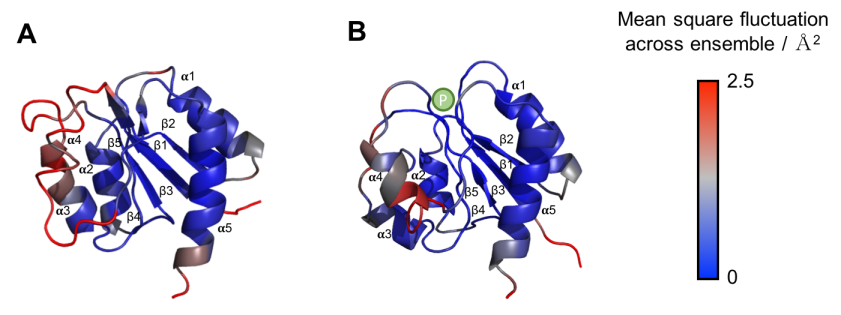
\includegraphics[width=0.9\textwidth]{figures/ntrc/ntrc}

\caption{Ensembles of NtrC.
(A) The mean square fluctuation in the unperturbed ensemble is shown on the inactive structure (PDB ID 1DC7).
(B) The mean square fluctuation in the ensemble with additional constraints representing phosphorylation is shown in the active structure (PDB ID 1DC8).
Labels are taken from \cite{Volkman2001}.}

\label{fig:ntrc}
\end{figure}


\section{Discussion}

The allosteric prediction methods PARS, STRESS and AlloPred all use NMA to predict allosteric sites.
NMA is computationally-inexpensive and hence suitable for high-throughput, automated approaches.
However the assumption of harmonic fluctuations around an energetically-minimum structure often makes prediction of conformational changes difficult, particularly for transitions with a low degree of collectivity \cite{Yang2007}.
In addition, the choice of which normal modes to use is non-trivial.
Larger conformational changes are associated with low-frequency normal modes but higher-frequency modes are also required to take into account local effects.
The focus of NMA on changes in dynamics is also important - whilst NMA-based methods might be expected to reveal perturbations to vibrations in proteins there are a variety of other motions that contribute to allostery, such as local unfolding and rigid body movements \cite{Motlagh2014}.
By contrast, ExProSE generates native-like protein structures that can span large conformational changes.
The structure generation process is then perturbed to predict allosteric sites.
This has the potential to discover effects not revealed by NMA-based methods, whilst retaining the low computational cost and ease of use.
It also provides an ensemble of structures under the influence of the predicted modulator that can be used, for example, in flexible ligand docking.
Energy minimisation provides a way to improve the stereochemistry of generated structures for use in such approaches.

ExProSE requires two structures for each protein, whereas other methods only require one.
It also requires the structures to be different from each other in order to generate structures that span the conformational space.
This makes the method unsuitable for use on proteins where only one structure, or highly similar structures, are available.
However, many medically-important proteins have multiple structures available, including the examples used in this study.
In these cases, it makes sense to use the additional structural information.
There are some methods which can predict holo structures from an apo input structure \cite{Seeliger2010, Grove2013} and these could be used to generate apo/holo pairs.
The method also was successful at reproducing the allostery in CAP using only one structure as input.
For proteins with multiple different conformational states, more than two structures could be used as input to ExProSE to explore further regions of conformational space - the constraint combination procedure can be applied to an arbitrary number of structures.

For many ensemble generation methods, such as MD and tCONCOORD, the choice of parameters has a large effect on the structures produced.
The parameter in ExProSE with the largest effect is $W_{B}$ (see the experimental procedures), which affects the conformational spread of the ensemble.
Without any user input, the auto-parameterisation step of ExProSE selects a value that gives an ensemble well-spread over the conformational space between the two input structures.
Once $W_{B}$ has been selected automatically, an ensemble that spans the correct space is generally produced without any further choice of parameters.
This makes the method suitable for high-throughput structure generation across multiple proteins as the user does not need to make any parameter choices themselves.
The auto-parameterisation procedure can be adjusted to obtain the desired level of structural flexibility using the parameter $F$, which is intuitive in terms of the spread of structures over conformational space (see the experimental procedures).
This provides a way to generate an ensemble with more flexibility if the input structures are similar, as mentioned above.

In this study, LIGSITE\textsuperscript{\it cs} was used to predict pockets for ExProSE.
However, it is worth noting that any pocket prediction method that outputs pocket points is compatible with ExProSE without modification.
One of the challenges in allosteric site prediction is discovery of transient pockets - pockets that are only present in some structures of the ensemble.
These pockets are an appealing target as they have thus far been unavailable to pocket prediction methods on crystal structures.
There are currently no general methods that use transient pockets for allosteric site prediction \cite{Boehr2009}, though recent studies have used Markov state models on MD simulations to predict cryptic allosteric sites on multiple proteins \cite{Bowman2012, Bowman2015}.
These studies concluded that cryptic allosteric sites are more ubiquitous than previously thought.
For example, transient sites were found on TEM-1 \textbeta -lactamase, which has been studied extensively without observing these sites \cite{Bowman2015}.
ExProSE has the potential to identify transient pockets and predict their ability as allosteric sites.
For example, an ensemble could be generated from apo/holo pairs and clustered into a few representative structures.
LIGSITE\textsuperscript{\it cs} could then be run on these structures to find potential transient pockets, and the perturbation procedure carried out to assess their allosteric character.
In intial tests of this approach, the known transient allosteric site on TEM-1 \textbeta -lactamase opened up in some representative structures from an ExProSE ensemble.
Methods for predicting pockets on an ensemble of protein structures, such as MDpocket \cite{Schmidtke2011} or the method in Polyphony \cite{Pitt2014}, could also be run on ensembles generated using ExProSE.

The results from ExProSE have implications for the conformational selection/induced fit debate \cite{Boehr2009}.
The principle of ExProSE is based on the conformational selection paradigm - an existing ensemble is perturbed by an effector to change the populations, as shown in Figure~intro fig.
% Is this really true?
This suggests that cases for which ExProSE is successful adopt a conformational selection mechanism.
The conformational selecion present in NtrC was reproduced by the method, for example.
In general this focus on conformational selection can be seen as a positive because small molecules binding with weaker interactions has been associated with a preference for conformational selection over induced fit \cite{Okazaki2008}, and it is these type of interactions that are important for allosteric modulator discovery.
It was found in some cases, however, that the additional constraints due to a predicted modulator caused the system to sample structures not present in the unperturbed ensemble.
% Any examples from figures?
This can be viewed as an induced fit effect, with the modulator binding allowing the ensemble to access structures which are not available in the absence of the modulator.
Study of perturbed ensembles using ExProSE could therefore give evidence for conformational selection or induced fit mechanisms in specific proteins.

ExProSE has the potential to be further improved.
Other numberical methods for satisfying the distance constraints could be explored, as there are many available \cite{DeBakker2006}.
The interactions used to generate distance constraints could be further refined; this was carried out for CONCOORD and gave slightly improved results \cite{DeGroot1999}.
Given the ease of automation of the whole pipeline, ExProSE has the potential to be turned into a web server.
Users could generate an ensemble of protein structures from one or two input structures, or predict allosteric sites from two input structures.
The ability of the method to generate structures for protein-protein docking or for flexible ligand docking could be explicitly investigated.
For example, structures generated from unbound protein interacting partners could be generated and docked to see if better binding models are produced.

ExProSE builds on existing methods by using more structural information as input.
It is able to generate ensembles of protein structures that span relevant conformational changes in proteins.
This makes it an effective alternative to similar methods and to MD, which it is often not feasible to run on timescales long enough to explore large motions of interest without specialist approaches.
The perturbation procedure can be applied systematically to predict allosteric sites.
In a comparison of multiple allosteric site predictors, ExProSE showed performance similar to and complementary with existing methods.
Experimental results in the well-studied CAP were also reproduced by ExProSE.
The ability to generate ensembles of protein structures and investigate the response of an ensemble to perturbations should prove useful for both the exploration of individual proteins and the systematic study of the whole PDB.
Such methods are required to make sense of the increasing volume of structural data, and to understand the crucial importance of dynamics to protein function.
